\documentclass[12pt, a4paper]{report}
    \usepackage[T1]{fontenc}
    \usepackage[utf8]{inputenc}
    \usepackage{pdfpages}
    \usepackage{float}
    \usepackage{listings}
    \usepackage{siunitx}   
    \usepackage{nicefrac}
    \usepackage{pifont}
    \usepackage{xcolor}
    \usepackage{amsmath}
    \usepackage[toc,nonumberlist]{glossaries}
    \makeglossaries
    \newglossaryentry{Rolling shutter}
    {
      name=Rolling shutter,
      description={When the camera needs to capture an image, it reads out pixels from the sensor a row at a time rather than capturing all pixel values at once}
    }
    
    \newglossaryentry{Balance wheel}
    {
      name=Balance wheel,
      description={is a wheel that regulates or stabilizes the motion of a mechanical watch and is responsible for the clock to run precisely}
    }
    
  \newglossaryentry{Time scale}
    {
      name=Time scale,
      description={is used to measure the rate deviation of a mechanical watch in different positions}
    }
    
    \newglossaryentry{SAD}
    {
      name=SAD,
      description={(sum of absolute differences) is a positive number, which results from the formation of the difference between two digital images. It serves as a measure of the difference between two images and is used in image processing and pattern recognition. It is obtained by subtracting the color values of the images pixel by pixel from each other and adding them up by amount}
    }
    
    \newglossaryentry{MMAL}
    {
      name=MMAL,
      description={(Multimedia Abstraction Layer) is a framework designed by Broadcom to provide a host-side, simple and relatively low-level interface to multimedia components running on the Videocore IV GPU on the Raspberry Pi}
    }
    
    \newglossaryentry{Optical Flow}
    {
      name=Optical flow,
      description={ of an image sequence is the vector field of the velocity projected into the image from visible points of the object in the reference system of the imaging optics}
    }
    
    \newglossaryentry{Codecvisa}
    {
      name=Codecvisa,
      description={is a powerful real-time analyzer for different video codecs
      http://www.codecian.com/}
    }
    
        \newglossaryentry{Rate Deviation}
    {
      name=Rate Deviation,
      description={is the difference between the measured period duration and the target period duration. From this it can be concluded how precisely the clock displays the time}
    }
    
  \newglossaryentry{VCHI}
    {
      name=VCHI,
      description={VideoCore Host Interface is a message passing system provided to permit communication between CPU and GPU \cite[ch. 6]{ReadTheDocsPicamera}}
    }
    
  \newglossaryentry{API}
    {
      name=API,
      description={application Programming Interface. Clear defined interface to communicate between components}
    }
    
      \newglossaryentry{DMA}
    {
      name=DMA,
      description={(Direct Memory Access) allows specific hardware systems of a computer system to access main system memory independently of the CPU \cite[p. 34 - 38]{Kuck1978}}
    }
    
          \newglossaryentry{CPU}
    {
      name=CPU,
      description={(Central Processing Unit) is the electronic circuitry in a computer, which executes the instructions of a computer program \cite[p. 36 - 38]{Kuck1978}}
    }
    
   \newglossaryentry{Photon}
    {
      name=Photon,
      description={is an elementary particle, which includes electromagnetic radiation (e.g. light) and moves at the speed of light within a vacuum \cite[ch. 31]{Halliday2005}}
    }

    \newglossaryentry{Motion blur}
    {
      name=Motion blur,
      description={motion blur is the apparent streaking of rapidly moving objects in a still image or a sequence of images such as a movie or animation}
    }

    \newglossaryentry{Raspberry Pi}
    {
      name=Raspberry Pi,
      description={is a credit-card-sized single-board computer for hobbyist and education use}
    }

    \newglossaryentry{GPU}
    {
      name=GPU,
      description={(graphics processing unit) is a specialized and optimized processor for calculating graphics}
    }

    \newglossaryentry{VideoCore IV}
    {
      name=VideoCore IV,
      description={is a multimedia processor low powered and optimized for image applications such as image compression and decompression}
    }
    
    \newglossaryentry{Processor}
    {
      name=Processor,
      description={is a computation unit}
    }
    
    
    \usepackage{booktabs}
    \usepackage{float}
    \usepackage{hyperref}
    \usepackage{mathtools}
    \hypersetup{
        colorlinks,
        citecolor=black,
        filecolor=black,
        linkcolor=black,
        urlcolor=black
    }
    
    \usepackage{tabularx}
        \newcolumntype{L}{>{\raggedright\arraybackslash}X}
     
     \usepackage[style=numeric, backend=biber]{biblatex}
     \bibliography{PA_cogsworth_citation}

     
    \begin{document}
    
    \begin{titlepage}
    
    \newcommand{\HRule}{\rule{\linewidth}{0.5mm}} % Defines a new command for the horizontal lines, change thickness here
    
    \center % Center everything on the page
    
    \textsc{\LARGE ZHAW School of Engineering}\\[1.5cm] % Name of your university/college
    \textsc{\Large Projektarbeit}\\[0.5cm] % Major heading such as course name
    \textsc{\large IT}\\[0.5cm] % Minor heading such as course title
    
    \HRule \\[0.4cm]
    { \huge \bfseries Measurement of Rate Deviation}\\[0.4cm] % Title of your document
      { \huge \bfseries  of Watches with Raspberry Pi Camera}\\[0.4cm] % Title of your document

    \HRule \\[1.5cm]
    
    
    \begin{minipage}{0.4\textwidth}
    \begin{flushleft} \large
    \emph{Authors:}\\
    Linda Helen \textsc{Boedi}  Valentin \textsc{Bossi} % Your name
    \end{flushleft}
    \end{minipage}
    ~
    \begin{minipage}{0.4\textwidth}
    \begin{flushright} \large
    \emph{Supervisor:} \\
    Hans-Joachim  \textsc{Gelke} % Supervisor's Name
    \end{flushright}
    \end{minipage}\\[2cm]
    
    
    {\large \today}\\[2cm] 
    
    
\includegraphics[scale=0.05]{Images/logo.png}\\[1cm] 
    
    \vfill 
    
    \end{titlepage}
    
    \pagenumbering{roman}
    
    \chapter*{Declaration of Autonomy}
     \addcontentsline{toc}{chapter}{Declaration of Autonomy}
     
     The undersigned certify with their signature that the work has been written independently and put into written form, that the involvement of other persons has been limited to consulting and proofreading, and that all documents and guarantors used are listed.

 \vskip4cm
$\overline{\hbox{\phantom{mmmm}Place and Date\phantom{mmmm}}}$\hskip2cm
$\overline{\hbox{\phantom{mmm}Linda Helen Bödi\phantom{mmm}}}$

\vskip3cm
$\overline{\hbox{\phantom{mmmm}Place and Date\phantom{mmmm}}}$\hskip2cm
$\overline{\hbox{\phantom{mmmm}Valentin Bossi\phantom{mmmm}}}$

\chapter*{Abstract}
 \addcontentsline{toc}{chapter}{Abstract}
Mechanical watches must be checked for clock drifts both during manufacture and use. Most of the equipment used for this purpose is expensive. Almost all of the devices on the market apply acoustic measurements and a few complement this measurement with an optical measurement done with a laser beam. In this the question has been tackled whether a Raspberry Pi and a Raspberry Pi camera can be turned into a cheaper and simple measuring device that can compete with the accuracy of a professional device using a new approach: image processing. 
\newline
The work will give answers to the following questions: Is an exclusive optical measurement by means of image processing possible? How accurate will these measurements be and can they keep up with the results of professional equipment? How can the measurement be further improved? 
\newline
In a first step, possible methods were evaluated in order to carry out the optical measurement of the frequency of the balance wheel of a watch. A closer look was taken at a one-to-one comparison of images, tracking a specific pixel, the OpenCV, the Gstreamer and the Picamera library. Since the Picamera library offers a very detailed documentation and many of the functionalities needed for this work, this library was used eventually. In order to better understand the motion vectors, various experiments were carried out, whereby the camera settings were also improved. Using the data from these experiments, an implementation of a Python program was carried out. The experiments also showed that the clock drift of the watch reacts very sensitively to varying temperatures, making it difficult to get reliable reference measurements. For this reason, a setup using a blinking LED with known frequency was chosen as a reference. The obtained results showed that the determination of the frequency by means of image processing worked very well and that sufficiently precise results could be achieved. In order to get better direct reference measurements, some meterings of a watch were done in parallel with the camera and a Greiner measurement device. It turned out that the results of both devices are very similar and therefore the measurement with the camera is accurate enough. For a precision of 5, 3, and about 2s one needs approximately 40s, 150s and 600s of measurement accordingly. In order to turn the presented approach into a product which can compete with the professional devices, some more implementations of measurements of various other things need to be made. Additionally, one could do further research, if real-time measurements are required.

\pagebreak
    \setcounter{secnumdepth}{5} 
    \setcounter{tocdepth}{5} 
    \pagenumbering{gobble}
    \tableofcontents
    \pagebreak
    \pagenumbering{arabic}
    
    \chapter{Introduction}
    Today's watch technology requires measuring instruments to perform a wide variety of measurements and analyses on almost all types of watches with great precision and reliability.
    Mechanical watches must be checked in production and service for their rate deviation.
    There are different techniques to measure this deviation: either acoustically and optically or only acoustically.

    
    The aim of this work is to develop a handy device that can visually measure the rate deviation using inexpensive and simple gear.
    To achieve this, an existing camera consisting of the best-known single-board computer Raspberry Pi and the corresponding camera from Raspberry Pi is used.
    The vision of this project is substitute real-time measurements of professional equipment with a much cheaper device. 


    The second chapter will give a background for this work. Acoustical and optical measurement will be explained and compared. One will have a look at the functionality and operation of mechanical watches and the camera module used in this project.


    In the third chapter different algorithms and libraries for image processing will be discussed and evaluated. 

    
    The test setup, camera settings and all methods used to get a better understanding of the Picamera library and motion vectors are listed in chapter four. 

    
    The fifth chapter explains how the frequency was calculated from the motion vectors and how it was implemented as a program in Python. 

    
    All measurements and results are listed in chapter six. A regression of the measurement error is discussed in chapter seven.

    
    The last chapter summarizes those results and outlines all the problems that occured during the work. It will also give an outlook of what could be improved and extended.

    \chapter{Background}
    This chapter is intended to lay the foundation for this report. An overview of the existing measuring methods for the accuracy of a mechanical watch is given and the Raspberry Pi camera, which was used for the optical measurements in this project, is described. In addition, the functionality of a mechanical watch is explained and important information about the test watch is listed.
    \section{State of the Art}
    At the beginning a small historical excursion, or rather an overview of the existing measuring methods for the accuracy of a mechanical watch is presented.
     \subsection{Optical versus Acoustical Measurement}
    There exist mainly two methods on the market to measure the frequency of the balance wheel of a mechanic clock; acoustical and optical measurement. The commonly used method is to analyse the beat noises of the lever escapement. More expensive devices use both acoustical and optical feedback. In order to classify the rate deviation well enough, it is usually measured in different positions of the watch.
    
    \subsubsection{Acoustical Measurement}
    The original method used for frequency measurements of the balance wheel is based on a vibrograph. For every "tick" of the clock a line was drawn onto a ongoing strip of paper. From the distance between of these lines the frequency was calculated \cite{Zeitwaage}. But as this method wasn't very accurate, other techniques have evolved.  
    Modern watch timing machines use an oscillating quartz crystal as comparison for the frequency of the balance wheel \cite{Zeitwaage}. The beat noises of the lever escapement are recorded and amplified with a microphone whereas unwanted background noises need to be filtered out. 
    
    \subsubsection{Optical Measurement}
    About hundred years later, optical watch timing machines joined acoustical ones. Even nowadays there are only a few devices on the market which employ only optical measurement, but several companies started to combine acoustical with optical metering. One way to determine the frequency of the balance wheel optically is by using a laser. The beam is periodically interrupted by the balance wheel and thus the frequency can be calculated \cite{Lombardi2011}. In this paper the frequency is quantified optically by using image processing. There is no known professional device which uses this technique for measuring the frequency.
    
    In table 2.1 a comparison of acoustical and optical measurements is made and the most important facts are listed.
    
        \begin{table}[H]
     \centering
    \begin{tabularx}{\linewidth}{ |c||L|L|  }
     \hline
     \multicolumn{3}{|c|}{\textbf{Comparison acoustical and optical measurement}} \\
     \hline
     & \textbf{acoustical}  & \textbf{optical} \\\hline
      since   &  around 19th century  \cite{Lombardi2011}  & end of 20th century  \cite{Lombardi2011}\\ \hline
     accuracy &   0.1 s/d & 0.1 s/d\\  \hline
     advantages & - most experience (exists for about 200 years) \newline - tracks if balance wheel is damaged (different noises) & - no background noises, which need to be filtered out\\  \hline
     disadvantages & - background noises need to be filtered out&- laser needs to be positioned precisely \newline- balance wheel needs to be visible  \newline - good lighting is needed\\
     \hline
    \end{tabularx}
    \caption{Comparison of Acoustical and Optical Measurement}
        \end{table}
        
    
    \subsection{Industrial Products}
     In the following section the three largest companies producing such measuring instruments are described and the most important facts are listed.
    \subsubsection{Witschi - WisioScope S}
    WisioScope S tests mechanical watches acoustically and optically. The measurement is done in parallel and is more accurate as two signals are used for the calculation of the frequency.
    The optical metering is done using a laser and lighting. A camera helps to adjust the watch properly. The price of their product is: CHF 10450.- .
    
    \subsubsection{Lepsi - WatchScope/WatchAnalyzer}
    The WatchScope and WatchAnalyzer from Lepsi are intended for watch lovers and are less suited for production. Both devices only work with an acoustic input with measurements of either a few seconds or up to 24 hours. All data can then be queried with the smartphone. WatchScope is the smaller, more convenient version. With the WatchAnalyzer you can measure the rate deviation of the watch in several positions. The prices for these products are CHF 369.- i.e. CHF 929.- .
    
    
    \subsubsection{Greiner Vibrograf - Compact 900}
    The Compact 900 measures the beat noises of the lever escapement. The price is CHF 4070.- .
    
    \bigskip
   The following table summarizes all important information for the three professional devices.
    
\begin{table}[H]
     \centering
    \begin{tabularx}{\linewidth}{ |c||L|L|L|  }
     \hline
     \multicolumn{4}{|c|}{\textbf{Measurement of rate deviation}} \\
     \hline
     &{\fontsize{9}{10}\selectfont \textbf{Witschi - WisioScope S}}  & {\fontsize{8}{9}\selectfont \textbf{Lepsi - WatchScope/WatchAnalyzer} }& {\fontsize{9}{10}\selectfont \textbf{Greiner Vibrograf - Compact 900} }\\\hline
      Scope   &  +/- 999.9 s/d  & +/- 1000 s/d &  +/- 1000 s/d \\ \hline
     Resolution &   0.1 s/d & 0.1 s/d & 0.1 s/d\\  \hline
     Price & CHF 10450.- & CHF 369.-, i.e. CHF 929.- &  CHF 4070.-\\  \hline
    \end{tabularx}
    \caption{ Measurement of rate deviation with different (semi-) professional devices}
 \end{table}
    
    \section{Camera Module}
    The documentation for the Picamera library \cite[ch. 6]{ReadTheDocsPicamera} provides a detailed introduction to the operation of the Raspberry Pi with camera, which is used for all measurements in this project. This chapter will briefly summarize this introduction to better understand the hardware and operation of the Raspberry Pi camera.
    
    As the original Raspberry Pi camera cannot record sharply small things and has no zoom, a lens was put in front of the camera. The camera module of the Raspberry Pi is basically a mobile phone camera module. Among other things, it uses a rolling shutter to take pictures. The pixel values of a frame are not captured completely at once, but are read line by line.
    
    However, the sensor is configured via the registers with the number of lines to be read and the corresponding time. The sensor reads the lines and pushes the data with the configured speed to the Raspberry Pi.
    
    This keeps the readout time of each line constant. However, the CPU does not "speak" directly to the camera, but the processing rather takes place on the GPU (VideoCore IV) of the Raspberry Pi which operates its own real-time operating system (VCOS).
    
    \bigskip
    \noindent
    \begin{figure}[H]
    \centering
    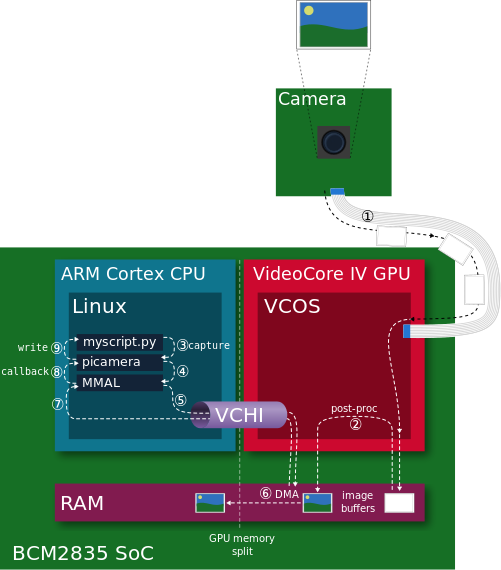
\includegraphics[scale=0.7]{Images/camera_architecture.png}
    
    \caption{Camera architecture \cite[ch. 6]{ReadTheDocsPicamera}}
    \end{figure}
    \bigskip
    
    Figure 2.1 illustrates the processing flow of a frame, with the associated steps explained in the following section.
    
    \begin{enumerate}
    \item The camera's sensor is configured and continuously streams frame lines to the GPU.
    \item The GPU builds complete frame buffers from these lines and performs the post-processing of these buffers.
    \item Myscript.py makes a capture call with the Picamera on the CPU.
    \item The Picamera library uses the MMAL API to meet this requirement.
    \item The MMAL API sends a message via VCHI requesting a frame capture.
    \item The GPU initiates a DMA transmission of the next full frame from its RAM portion to the CPU portion.
    \item The GPU sends back a message via VCHI that the capture is complete.
    \item This causes an MMAL thread to trigger a callback in the Picamera library, which in turn retrieves the frame.
    \item Picamera calls "write" on the output object provided by myscript.py.
    \end{enumerate}
    
    \subsection{Exposure Time}
    
    The camera sensor detects how many photons hit the sensor elements, because the more impact, the more they increase their counter values. The sensor can perform exactly two operations: reset a set of elements or read a set of elements.
    
    \subsubsection{Minimal Exposure Time}
    
    Reading out a series of elements takes a certain amount of time, thus there is a limit to the minimum exposure time. Assuming one has 500 lines on a sensor and reading each line takes at least 20ns, then it will take at least $500*20 \text{ns} = 10 \text{ms}$ to read a full screen. 
    
    \subsubsection{Maximum Framerate}
    
    The frame rate is the number of frames the camera can capture per second. The exposure time determines the maximum number of images that can be taken in a given time. Assuming it takes 10ms to read a complete image, then no more than $\frac{1 \text{s} }{10 \text{ms}} = \frac{1\text{s}}{0.01\text{s}} = 100 $ images are read in one second. 
    
    \bigskip
    
    The formula used reads as: 
    \begin{displaymath}
    \frac{1\text{s}}{\text{min exposure time in s}} = \text{max framerate in
    fps.} 
    \end{displaymath}
    The lower the minimum exposure time, the higher the maximum frame rate and vice versa.
    
    \subsubsection{Maximum Exposure Time}
    To maximize shutter speed, the framerate needs to be reduced. 
       \newline
      
        \bigskip
    Therefore the following is valid :
    \begin{displaymath}
    \frac{1\text{s}}{\text{min framerate in fps}} = \text{max exposure time
    in s}
    \end{displaymath} 
    
    \subsection{Hardware Limits}
    
    \begin{itemize}
    \item The Picamera originally has a very limited zoom. To record the watch properly a lens was added to the camera.
    \item The maximum horizontal resolution for the standard H264 recording is 1920 (this is a limitation of the H264 block in the GPU).
    \item The maximum frame rate of the camera depends on several factors. With overclocking 120 fps can be achieved, but 90 fps is the maximum supported frame rate.
    
    \end{itemize}
    
    \section{Mechanical Watches}  
    In the following, the function of a mechanical watch is explained in more detail and the role of a watch's balance wheel is explained. Subsequently, important information on mechanical watches, such as the duration of stroke and facts about the test watch used in this project, are described.
    \subsection{Operation of a Mechanical Watch}  
    In Figure 2.2 the components of a mechanical watch are illustrated. If a mechanical watch is wound up using the crown, the locking wheel (3) is moved by the winding shaft (1) and winding wheels (2). It turns the spring core (4) and pulls the tension spring in the mainspring barrel (5). The spring transmits the stored energy via the external toothed mainspring barrel (5) to the minute wheel (6), third wheel (7) and fourth wheel (8). 
    \newline
    \noindent
    \begin{figure}[H]
    \centering
    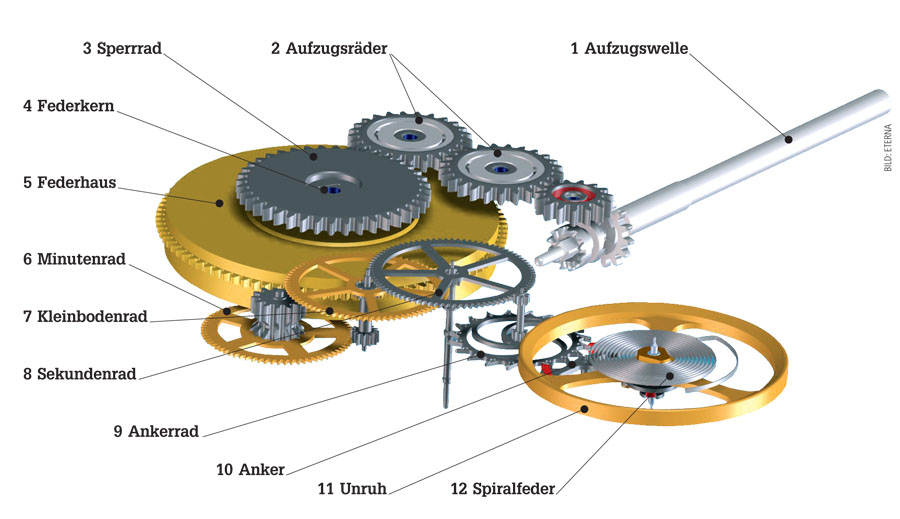
\includegraphics[scale=0.45]{Images/Funktionsweise-Uhrwerk.jpg}
    
    \caption{Operation of a mechanical watch \cite{Uhrwerk}}
    \end{figure}
    
The so-called escapement ensures that the gear train runs at the correct speed. The fourth wheel (8) drives the escape wheel (9); it gives an impulse to the pallet fork (10) which it passes on to the balance wheel (11), after which the armature, which moves back and forth like a seesaw, blocks the escape wheel. The balance wheel rotates, but is then retracted by the hairspring (12). It moves the armature back, which now releases the armature wheel again a little bit giving the armature with its rotation the next impulse. Due to the sudden braking and acceleration of the escapement wheel, the second hand of a mechanical watch also moves stepwise \cite{Uhrwerk}.
    \newline
    \noindent
    \begin{figure}[H]
    \centering
    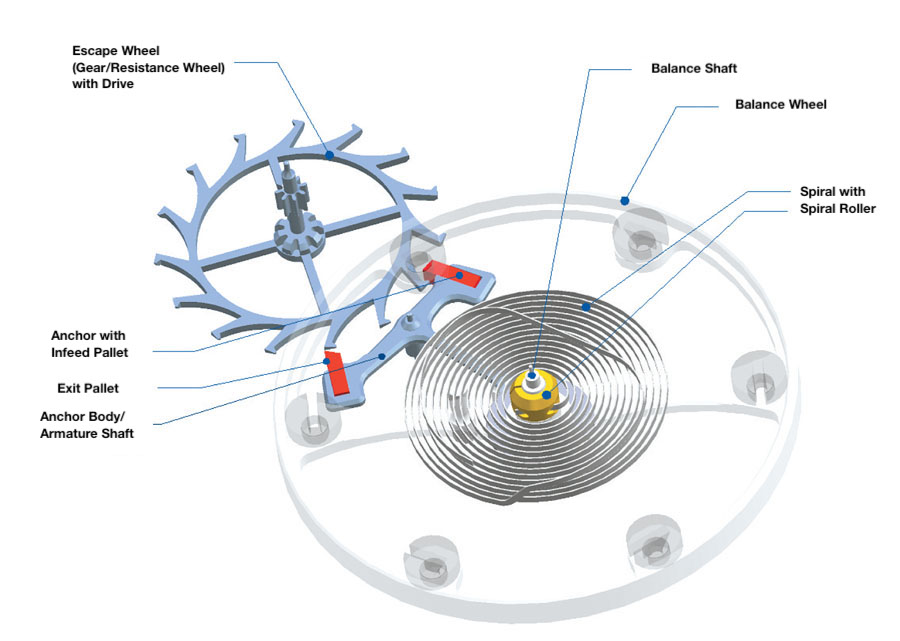
\includegraphics[scale=0.45]{Images/Hemmung-Teil1.jpg}
    
    \caption{Lever escapement and balance wheel \cite{Uhrwerk}}
    \end{figure}
\bigskip
The balance wheel, which is shown in Figure 2.3, is the heart of the oscillation system. It generates a time-defined movement which in turn is transferred to the gear train and passed on to the watch hands. 
The occurring error, if the balance wheel does not run accurately, is called rate deviation. The deviation can be caused by different external and internal matters. Internal motives often are wear, i.e. erosion or dirt. There are a lot more external causes like changes in temperature, air pressure or magnetism.

\subsection{Oscillation of the Balance Wheel}
In the following section, the movement of the balance wheel, which will be recorded and used for the calculation of the frequency, is explained.

\subsubsection{Period}
The period of the balance wheel is the path of a point from one turning point to the other and back (A - B - A) as shown in figure 2.4 \cite[p. 9]{Witschi_basics}.
    \begin{figure}[H]
    \centering
    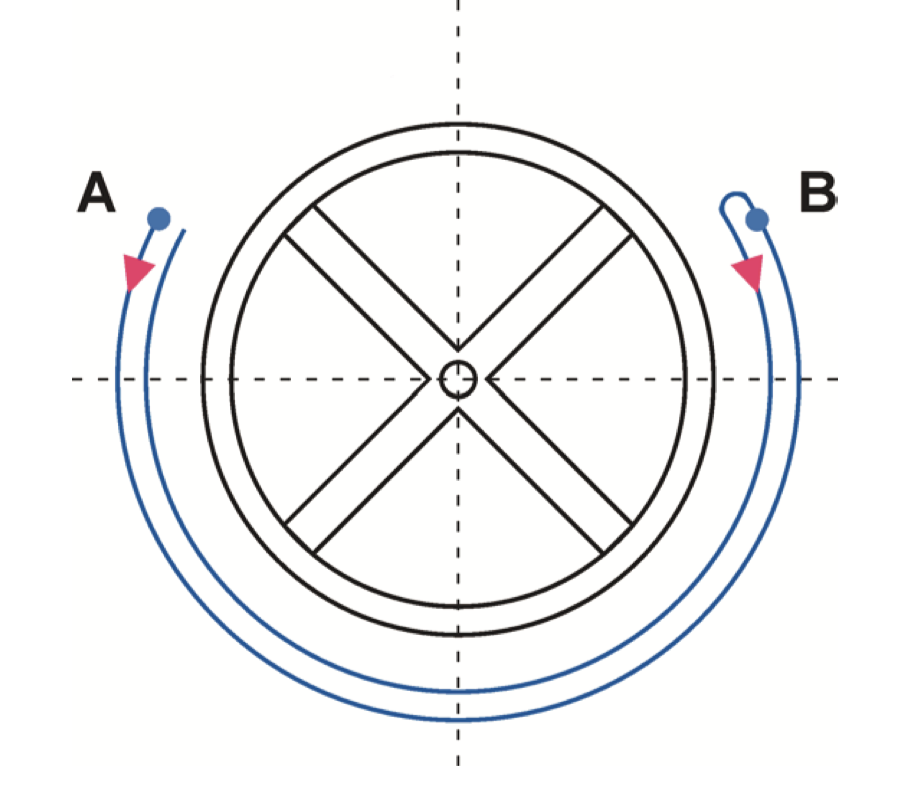
\includegraphics[scale=0.4]{Images/period.png}
    
    \caption{Period of the balance wheel \cite[p. 9]{Witschi_basics}}
    \end{figure}
\bigskip

\subsubsection{Half a Period}
In Figure 2.5 half of a period, i.e. one stroke, of the balance wheel is illustrated. It is the path of a point from one turning point to the other (A - B) \cite[p. 9]{Witschi_basics}.
    \begin{figure}[H]
    \centering
    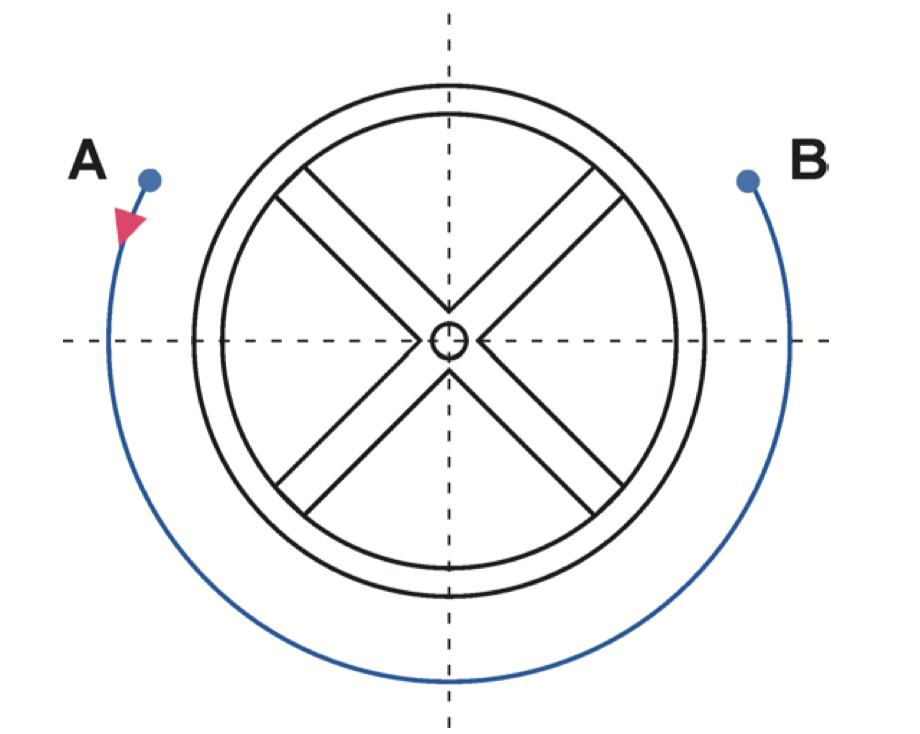
\includegraphics[scale=0.4]{Images/Halfperiod.png}
    
    \caption{Half of a period of the balance wheel \cite[p. 9]{Witschi_basics}}
    \end{figure}
\bigskip
    
    \subsection{Number of Strokes}
    Since the rate deviation has been calculated in seconds per day and the number of strokes per hour, i. e. the number of audible impulses of a two-armed pallet fork of a mechanical watch per hour, is known, these two quantities must first be expressed in a common unit. The relationship between the number of strokes (n*) and frequency (f) is as follows \cite{Krug1987}: 
    
    \begin{displaymath}
    n\text{*} = 2f*3600
     \end{displaymath}
     and therefore:
     \begin{displaymath}
      f = \frac{n\text{*}}{7200}
     \end{displaymath}
     
     \bigskip
     
    The following table lists important facts about mechanical wristwatches. Among other things, it contains the number of strokes per hour, the duration for one stroke, i. e. half a period, and the frequency.
    
     \begin{table}[H]
     \centering
    \begin{tabularx}{\linewidth}{ |L|L|L|L|L|  }
     \hline
     \textbf{Number of strokes} (1/h) &  \textbf{Stroke duration} (s)& \textbf{Oscillation number}  (1/h)& \textbf{Period duration} (s)& \textbf{Frequency} (Hz)\\\hline
      18'000   &  0.200  & 9'000 & 0.400 & 2.50\\ \hline
     19'800 &  0.182 & 9'900 & 0.364 & 2.75\\  \hline
     21'600 &  0.166 & 10'800 & 0.333 & 3.00\\  \hline
    28'800 &  0.125 & 14'400 & 0.250 & 4.00\\  \hline
    36'000 &  0.100 & 18'000 & 0.200 & 5.00\\  \hline
    \end{tabularx}
       \caption{  Number of strokes, period duration and frequency of the balance of automatic wristwatches \cite{Krug1987}}
        \end{table}
        
        \subsection{Test Watch}
      The test watch, which was used, is of the caliber ETA C01.211. It is a chronograph with a diameter of 31 centimeters. It strokes 21600 times per hour with a stroke duration of 0.1666 seconds. It therefore has a frequency of 3 Hz. Additionally, the watch has a power reserve of 43 hours \cite{Caliber}.

    \chapter{Technologies and Algorithms}
 The investigation of image processing packages comprised three libraries:
 \begin{enumerate}
 \item OpenCV
 \item Gstreamer
 \item Picamera
 \end{enumerate}
\textbf{OpenCV} is an open source library which is suitable and widely used for the programming languages C++, C, Python and Java. It combines different algorithms for image processing and machine vision. It offers modules that implement algorithms which can solve common problems such as face recognition, gesture recognition, object recognition, tracking and optical flow, to name but a few \cite{opencv}.
\bigskip

\textbf{Gstreamer} is another open source library, mainly programmed in C. As the name suggests, this library is mainly used for multimedia data streams such as media players and video editing software \cite{gstreamer}.

\bigskip
The last library, \textbf{Picamera}, is again an open source project sporting a Python API. The library is an interface to the MMAL (written in C) which in turn is an interface to the firmware of the GPU. This means that the camera can be accessed using a simple programming language such as Python. The Picamera library is very strongly tailored to the raspberry pi camera, but offers a wide range of functionalities \cite[ch. 1]{ReadTheDocsPicamera}.
    
    \section{Optical Flow}
    The optical flow represents the vector field of the velocities of the points of an image sequence. It is a useful representation of motion information in image processing. The local optical flow is an estimate of patterns in an image in the vicinity of a viewed pixel. 
    
    One possibility would be to follow the course of a velocity vector and thereby calculate a period of the motion of the balance wheel. The calculation of the flow at selected points is also called feature point tracking. Another approach would be to calculate the frequency based on the velocity obtained from the optical flow, since it is more or less a circular movement. 
    
    One difficulty with this procedure is that one has to focus on certain pixels. This can cause problems if the clock is placed differently, because wrong points can cause problems for the calculation. In the worst-case scenario points, in which movement never takes place, would be examined.
    
    \subsection{Sparse Optical Flow}
    
    The OpenCV library uses the Lucas-Kanade method to calculate the optical flow. The Lucas-Kanade method also assumes that the flow in the local environment of the pixel for which the flow is intended is the same as the one of the pixel. So more or less a whole set of pixels is considered. The flow can thus be determined by calculating the derivatives (= gradients) \cite{opencv}.
    
    One characteristic of this method is that it does not provide a dense flow. This means the flow information disappears quickly with the distance from the edges of the image. The advantage of the method is its relative robustness against noise and smaller defects in the image.
    
       \subsection{Dense Flow}
The dense optical flow calculates the flow over all pixels of an image, so the whole image is processed. This method is more accurate than the sparse optical flow method, but also much slower.

The implementation in Open CV is based on the Gunner Farneback's algorithm which is explained in "Two-Frame Motion Estimation Based on Polynomial Expansion" by Gunner Farneback in 2003 \cite{Farneback2003}.
  
   \section{Kalman Filtering} 
   Using the Kalman filter, errors in real measurement values can be reduced and estimates for unmeasurable system variables can be provided. For this purpose, the values which are to be examined in more detail are described by a mathematical model, for example in the form of equations of motion. The special mathematical structure of the Kalman filter makes it possible to use it in real-time systems in different areas, such as the evaluation of GPS data to determine the position of moving objects (tracking) or for augmented reality \cite[ch. 1.2]{Grewal1993}.
   
   \section{Object tracking}
   Object tracking, also called video tracking, is a process in which a moving object is tracked in a video. To achieve this, not only an algorithm for object tracking is used, but also an algorithm for object detection. Depending on the application, this process is computationally intensive. This procedure could be used to track the movement of the balance wheel and find out how fast it moves and when it stops \cite{objectTracking}.
    
 \section{Motion vectors}
 Motion vectors are used in video compression to reduce resources required to store and transmit data. A motion vector describes the displacement of a pixel or pixel block within an image sequence \cite{Motionvector}. 
 The motion vectors can be used to describe how much change is taking place in an image sequence. This can be used to identify a moving or still balance wheel.
    
   
   \section{Conclusions and Evaluations}
   Because in this project a mini computer is used and a realtime measurement is to be made, many presented technologies and algorithms are already excluded because they are computationally too expensive.
   This means that at 90 frames per second, a calculation on the image data must be done within \nicefrac{1}{90} seconds, no matter how computing-intensive it is.
   In addition, there is the problem with object tracking, for example, that there are many different shapes of balance wheels and that the software would have to be adapted for each new shape of balance wheel in order to make the object detection work.
   The same applies to procedures that work with colors. As soon as a balance wheel has a different color, the procedure would have to be adapted.
   
   In Table 3.1 it is listed which methods are already implemented in which library, how high the computational effort is and if it is generalizable, so that the measurements are always more or less the same and the camera does not need to be positioned precisely in the exact same position every time.
  
   \begin{table}[H]
    
      \centering
        \begin{tabularx}{\linewidth}{|X|X|X|X|X|X|X|X|X|X| }
        \hline
         \multicolumn{3}{|c}{} & \multicolumn{1}{|c|}{\textbf{OpenCV}} & \multicolumn{1}{|c|}{\textbf{Gstreamer}} & \multicolumn{1}{|c|}{\textbf{Picamera}}\\\hline
       \textbf{}&   {\fontsize{8}{10}\selectfont Generaliz-ability }&  {\fontsize{8}{10}\selectfont Computa-tional Intensity} &   \multicolumn{3}{c|}{\fontsize{8}{10}\selectfont Implemented and Easy Accessible} \\ \hline
        {\fontsize{8}{10}\selectfont Optical Flow}           & \ding{51}        & high & \ding{51}    & \ding{55}  & \ding{55}\\ \hline
        {\fontsize{8}{10}\selectfont Kalman \newline Filtering}     & \ding{51}        & high     & \ding{51} &  \ding{55}          & \ding{55}\\ \hline
        {\fontsize{8}{10}\selectfont Object Tracking}     & \ding{51}        & high   & \ding{51}     & \ding{55}    & \ding{51}\\ \hline
        {\fontsize{8}{10}\selectfont Motion \newline Vectors and SAD} & \ding{51}  & very low  & \ding{55}   & \ding{55} & \ding{51}\\ \hline
      \end{tabularx}
    \caption{Evaluation of Different Algorithms}
    \end{table}
    
    As the computational effort is relatively low for the Picamera library and the motion vectors are already preprocessed and easy accessible, this library was chosen for the calculation of the frequency of mechanical watches.

    \chapter {Experimental approaches}

    After deciding which library to use, some experimental sessions took place to get a better understanding of the so called motion data values or motion vectors. 
    With the Picamera library it is easy to access these motion data values so the hard part was not data access but the understanding of how they are constructed. 
    The motion data object from Picamera consists of multiple values: a signed 1-byte x vector, a signed 1-byte y vector and and unsigned 2-byte SAD value for each macro-block of 16x16 pixels of a frame.
    
   \section{Test setup}
   
Figure 4.1 shows the test setup. On average, the camera was positioned approximately four centimeters from the test watch. In order to ensure that the images are still well illuminated and a good measurement can be carried out due to the high shutter speed, a small light source directed at the test watch was used. The test watch was positioned on a turn table so it was easy to adjust the position of the watch.

      \begin{figure}[H]
        \centering
        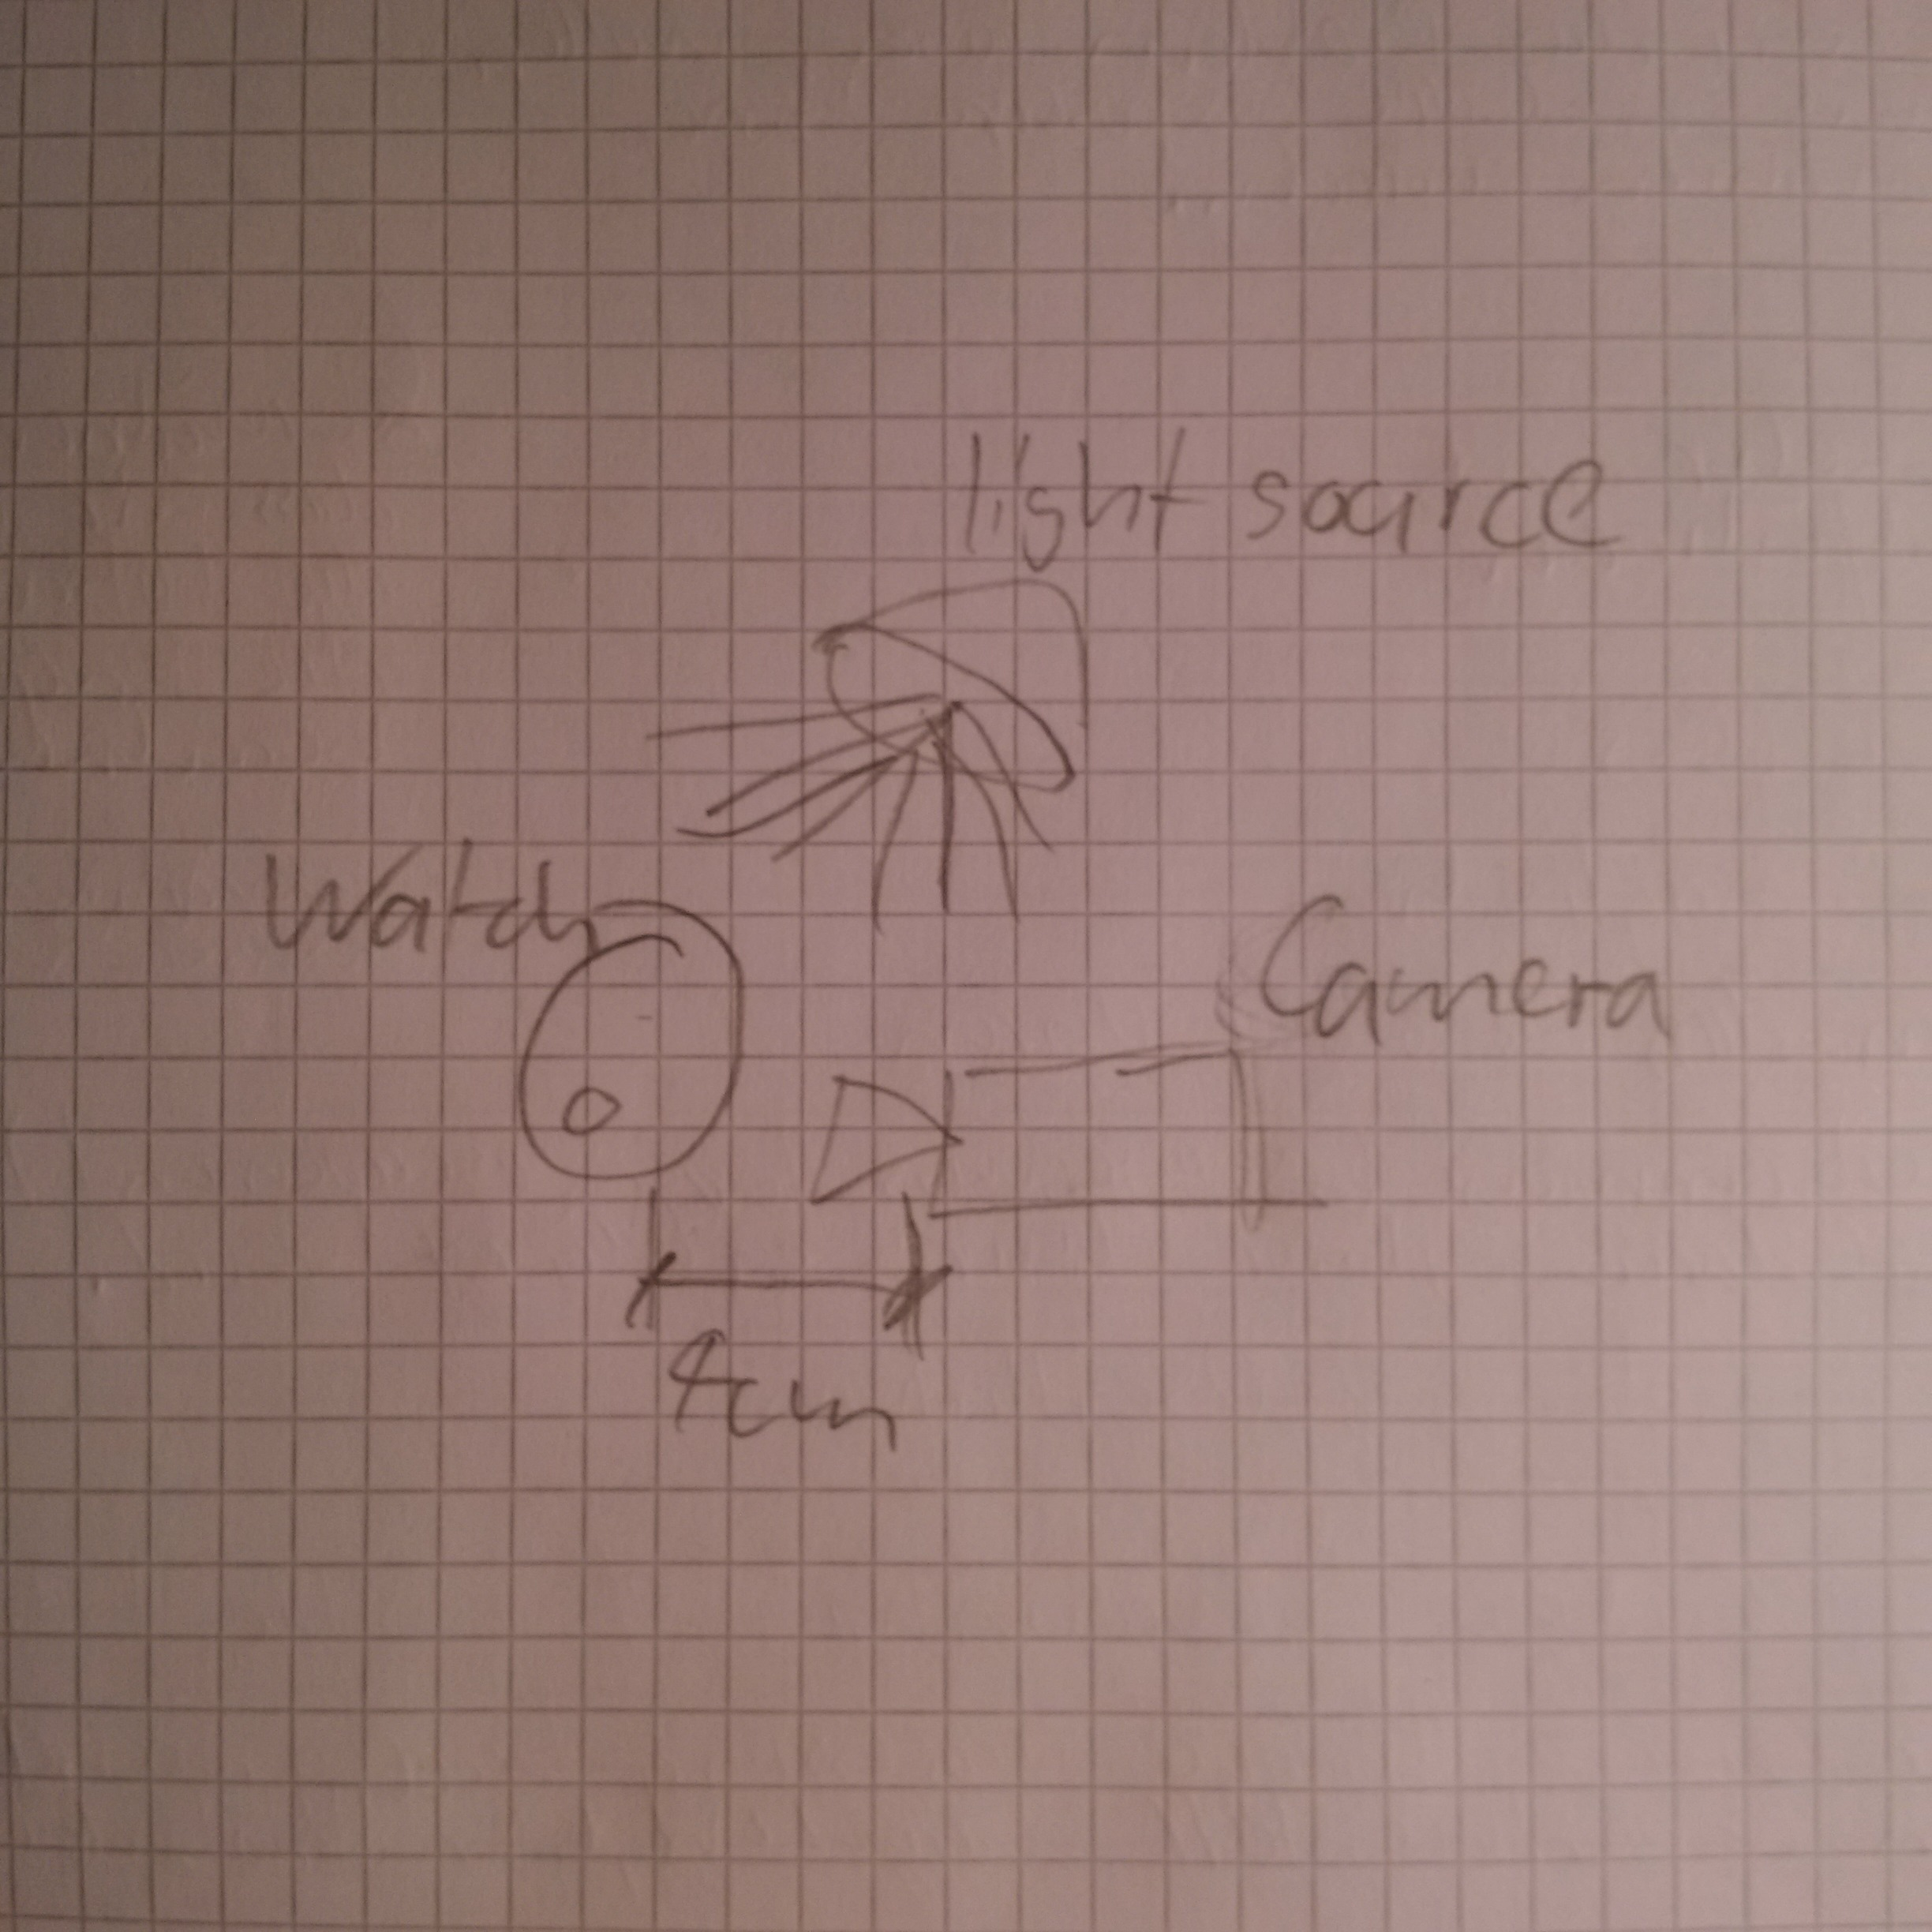
\includegraphics[scale=0.3]{Images/test_setup}
        
        \caption{Test setup for records}
        \end{figure}
        
    \section{Gesture Detection}
   In a first attempt, the hand in front of the camera was moved down, up, right and left in order to determine the direction in real time based on the motion vectors. 
    \newline
    For this, the average of all x-values and all y-values of the motion vectors of a frame are calculated and compared with a minimum value of movement that was defined. Depending on whether the x-average value is lower or higher than said minimum, a movement to the left or right has been detected. Likewise, it works for the y-average with the movement up or down.
        \newline
 As this worked quite well, the balance wheel of the test watch was recorded. Unfortunately, this program can only detect very clear movements. With very small movements this program fails, therefore the frequency of the balance wheel could not be calculated with this implementation. 
    
    \section{Animation of Motion Vectors}
    
   Another approach was to animate all SAD values with colors to determine whether they can be used to calculate the frequency of the movement of the balance wheel. In Figure 4.2 a snapshot of the animation of the SAD values is shown. The lighter the color of a pixel, the higher is the value of the SAD. 
    
    \noindent
    \begin{figure}[H]
    \centering
    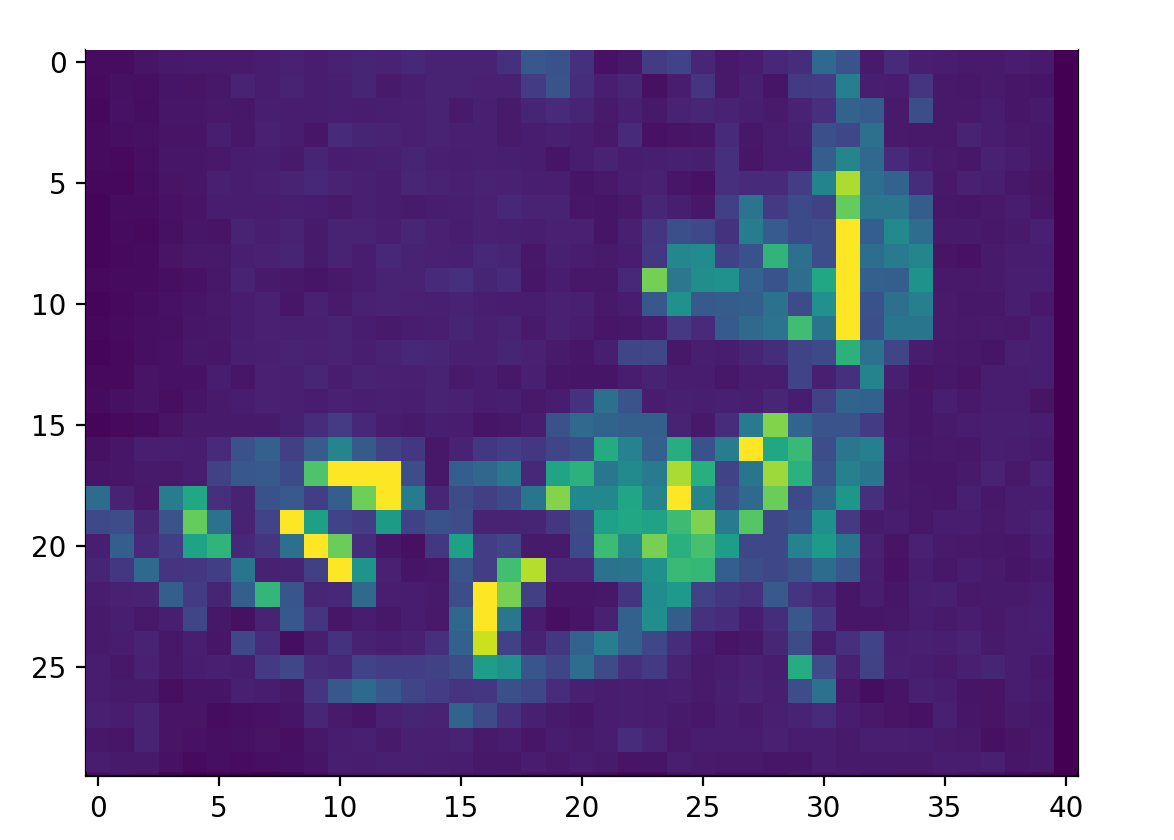
\includegraphics[scale=0.6]{Images/animation_sad.png}
    
    \caption{Snapshot of the animation of the SAD values}
    \end{figure}
     
    Furthermore, the x and y vectors were analyzed. But as those vectors itself are hard to use and only give partial information (y-vector: up or down, x-vector: right or left), the hypotenuses were calculated with Pythagoras' theorem and displayed similar to the SAD values as displayed in Figure 4.3. The hypotenuses give information about the amount as well as the direction of the motion. The lighter the color of a pixel, the higher the value of the hypotenuse.
 
        \noindent
    \begin{figure}[H]
    \centering
    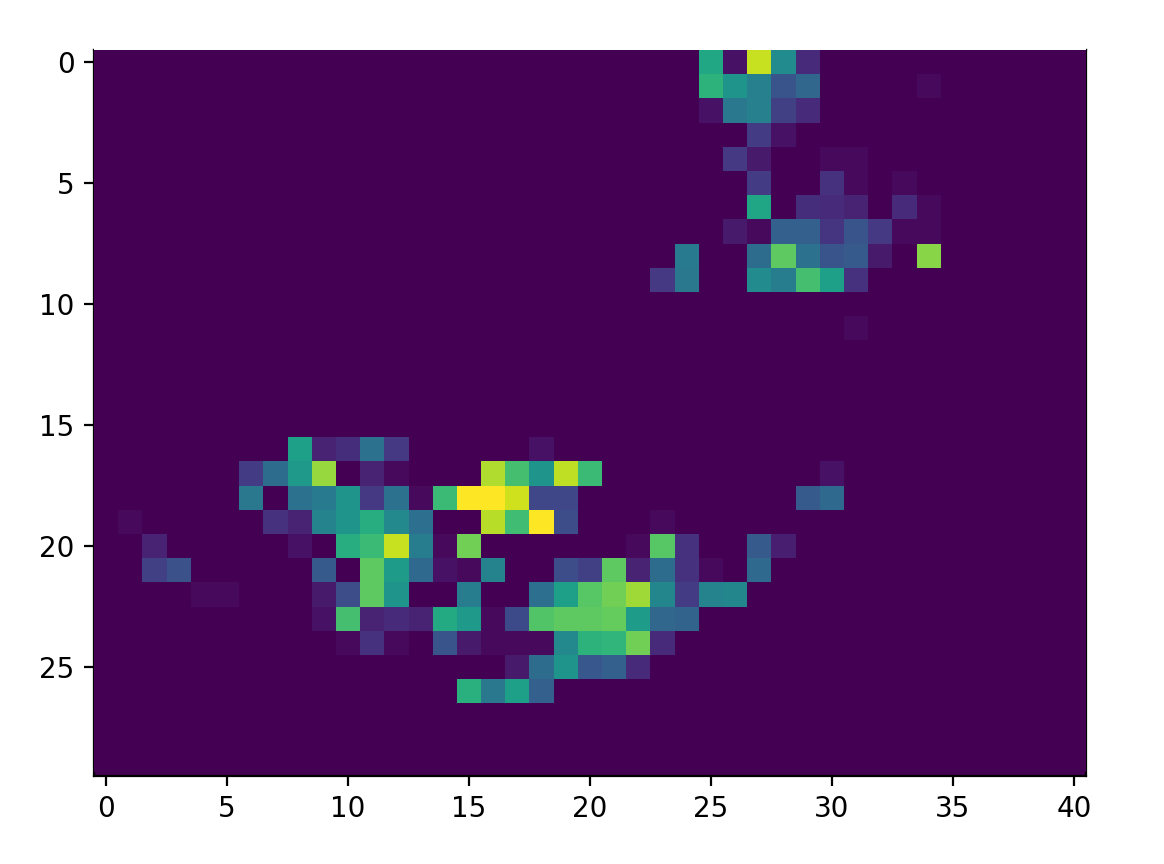
\includegraphics[scale=0.6]{Images/animation_hypotenuse.png}
    
    \caption{Snapshot of the animation of the hypotenuses}
    \end{figure}
    
    \pagebreak
    
    \section{Motion Vectors Visualized in a Frame}
        Another experimental approach was displaying the motion vectors as arrows directly in the video. This approach was helpful to get a better understanding of the conditions that yield the best result of the motion vectors.
    Codecvisa was used to display the motion vectors of a frame as arrows. The larger the arrow, the faster is the motion of this pixel. As one can see in Figure 4.4 the movement of the balance wheel is detected very well, as the arrows are bigger there.
 
    \noindent
    \begin{figure}[H]
    \centering
    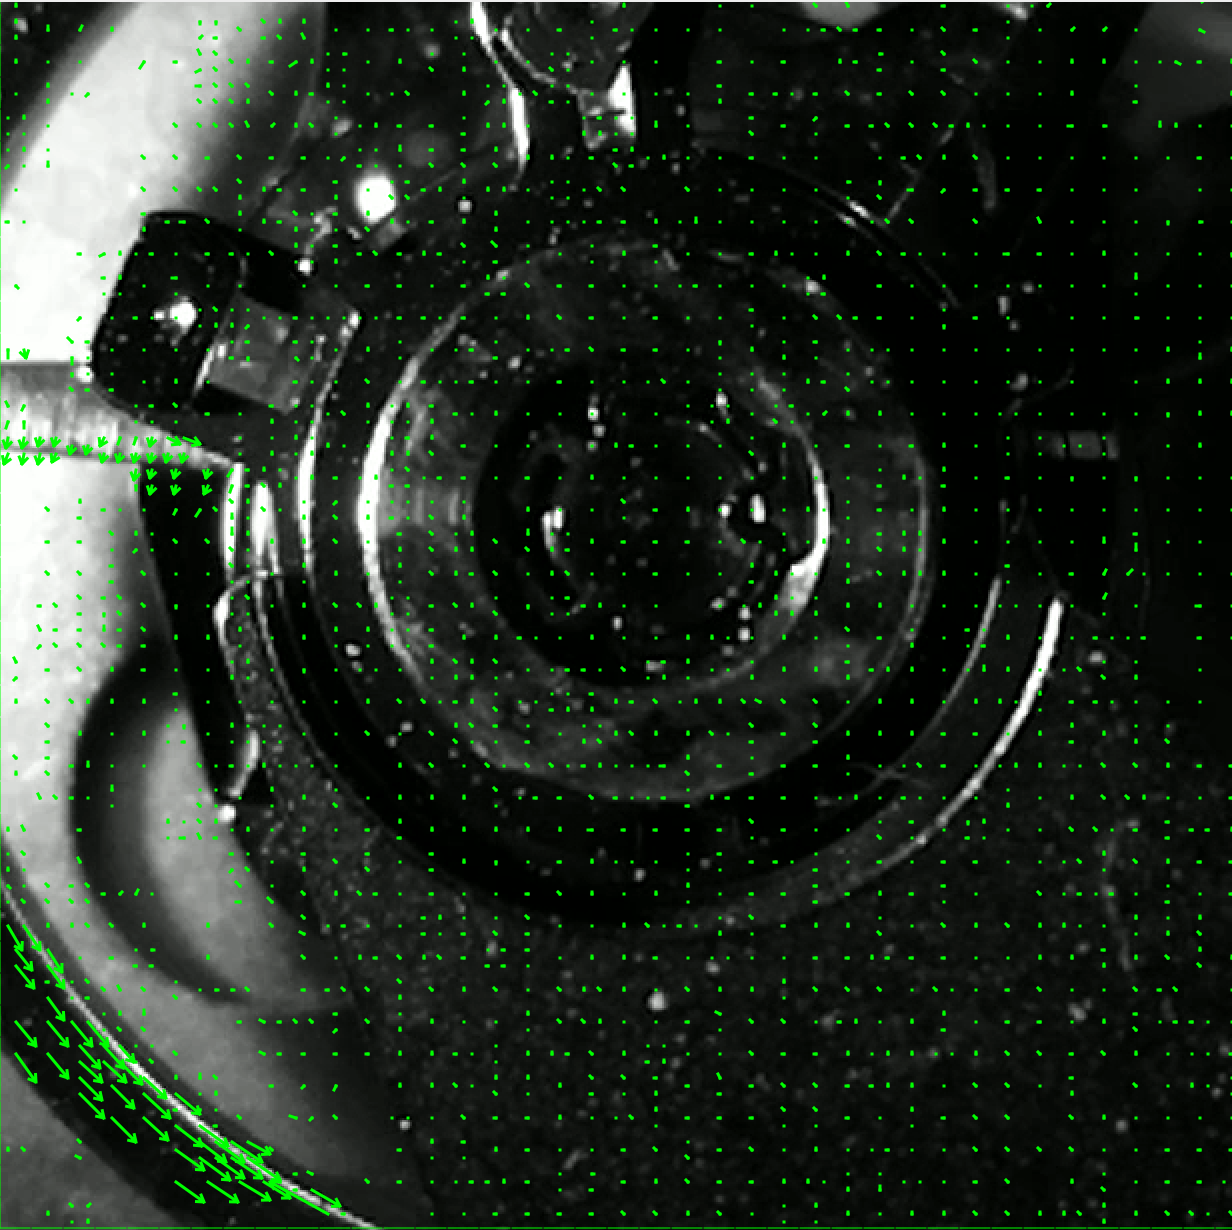
\includegraphics[scale=0.5]{Images/motion_vectors.png}
    
    \caption{Motion vectors drawn in one frame}
    \end{figure}
    
    \section{Analysis of Motion Vectors in Excel}
    Another approach used Excel was to determine whether a motion vector from one frame is the predecessor of the motion vector in the next frame.
    The hope was that a moving pixel could be followed and therefore the location of the pixel would always have been known.
    
     \begin{figure}[H]
    \centering
    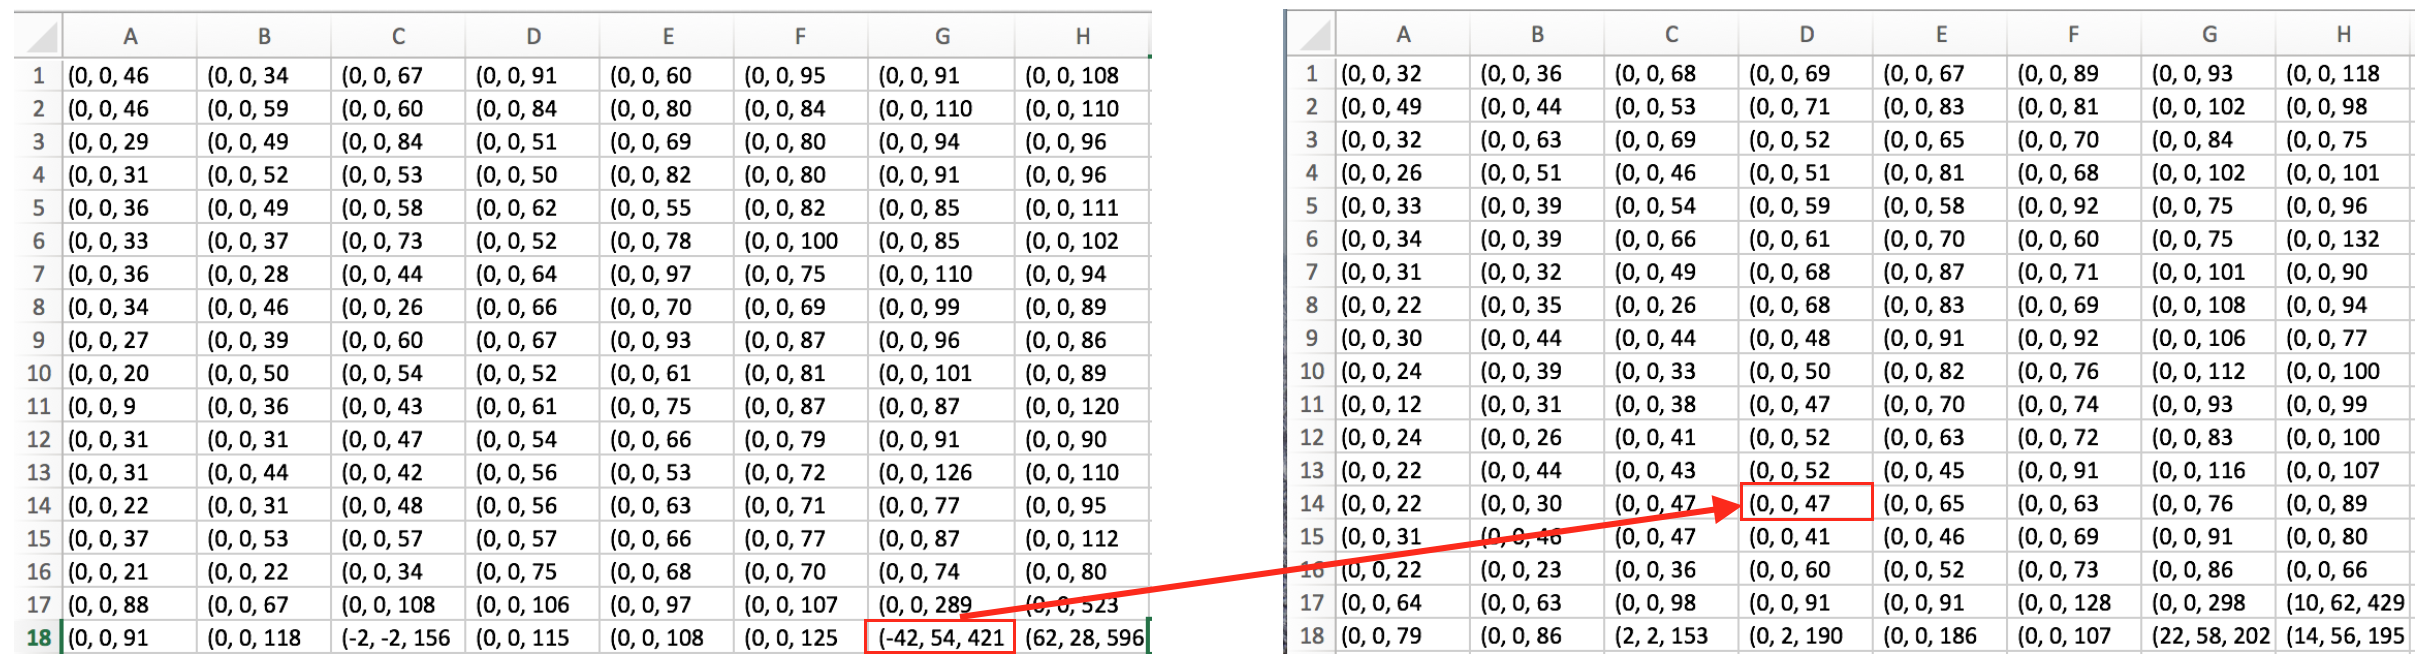
\includegraphics[scale=0.32]{Images/analysis_mv_excel.png}
    
    \caption{Motion vectors drawn in one frame}
    \end{figure}
    
    Two successive frames are illustrated in figure 4.5. Every field with the three values x, y and sad represents a 16x16 macro block. The idea was to calculate from those values where the pixel will be in the next frame. For example the field G18 contains -42 and 54 as x- and y-values. If those values are divided by 16, as the macro block has a size of 16x16, the idea was to add those resulting values rounded to the current field to get the next field, where this macro block might have moved. This is displayed as the red field, D14, in the right excel snippet. From the fields with high values in it, which is an indicator for a lot of movement, it was expected to get the movement of the balance wheel. 
    The result was sobering because one frame and motion vector cannot be associated with another frame and motion vector.
    This experiment is based on the idea of the optical flux with the movement vectors of the MMAL (Multi-Media Abstraction Layer) as displayed in Figure 4.6 .
    
    \noindent
    \begin{figure}[H]
    \centering
    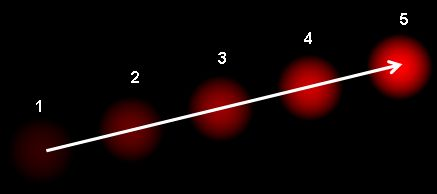
\includegraphics[scale=0.7]{Images/optical_flow_basic1.jpg}
    
    \caption{It shows a ball moving in 5 consecutive frames. The arrow shows its displacement vector.}
    \end{figure}
    
    \section{Influences of Camera Setup and Parameters}
    Testing with different settings showed that the results can be improved. For example, the black and white records are the best choice. Reducing the shutter speeds can reduce motion blur, which also contributes to a better result.
    The consequence of the shorter exposure time is that the light source must be very strong and close to the subject, otherwise the image is too dark and has a negative effect on the result.
    Records with changed angles were also taken. The angle was changed by about 30 degrees. With this adjustment, no significant changes in the measured values could be detected.
    Furthermore, it was recognized that the selected image detail influences the measured values. During the video recordings it was taken care that the balance wheel takes up the entire image.
    \newpage
    
    \chapter{Calculation of the frequency}
During the experimental sessions with the motion vectors it became clear how the information contained in the motion vectors could be used to calculate the oscillation of the balance wheel. At first, a crude calculation was made in Excel and the gained insights were then used to start implementing a program in Python. The following chapter will explain how those calculations and implementations were done.
    
     \section{Calculation of Frequency in Excel}
    With the help of the motion vectors and the corresponding time stamps per frame, a rough calculation of the frequency can be made. All x, y or SAD values contained in the image are summed up. If the sum of all values is small, it is very likely that the balance wheel is at a standstill before turning back again. For small values, the time stamp is registered and the difference to the next standstill is calculated. Since the balance wheel triggers half a oscillation, it has moved from one stop to the next half point. 
    In order to roughly calculate the frequency, an Excel sheet was created - Figure 5.1 is a snippet - in which all the accumulated absolute x- and y-values were entered and the standstills of the balance wheels were determined by eye. The half-oscillations and the frequency were calculated from the time intervals of the standstills. Afterwards, the average of all calculated frequencies was determined and it was recognized that the results with this method should be good enough to determine the frequency and thus the rate deviation. 
    
    \noindent
    \begin{figure}[H]
    \centering
    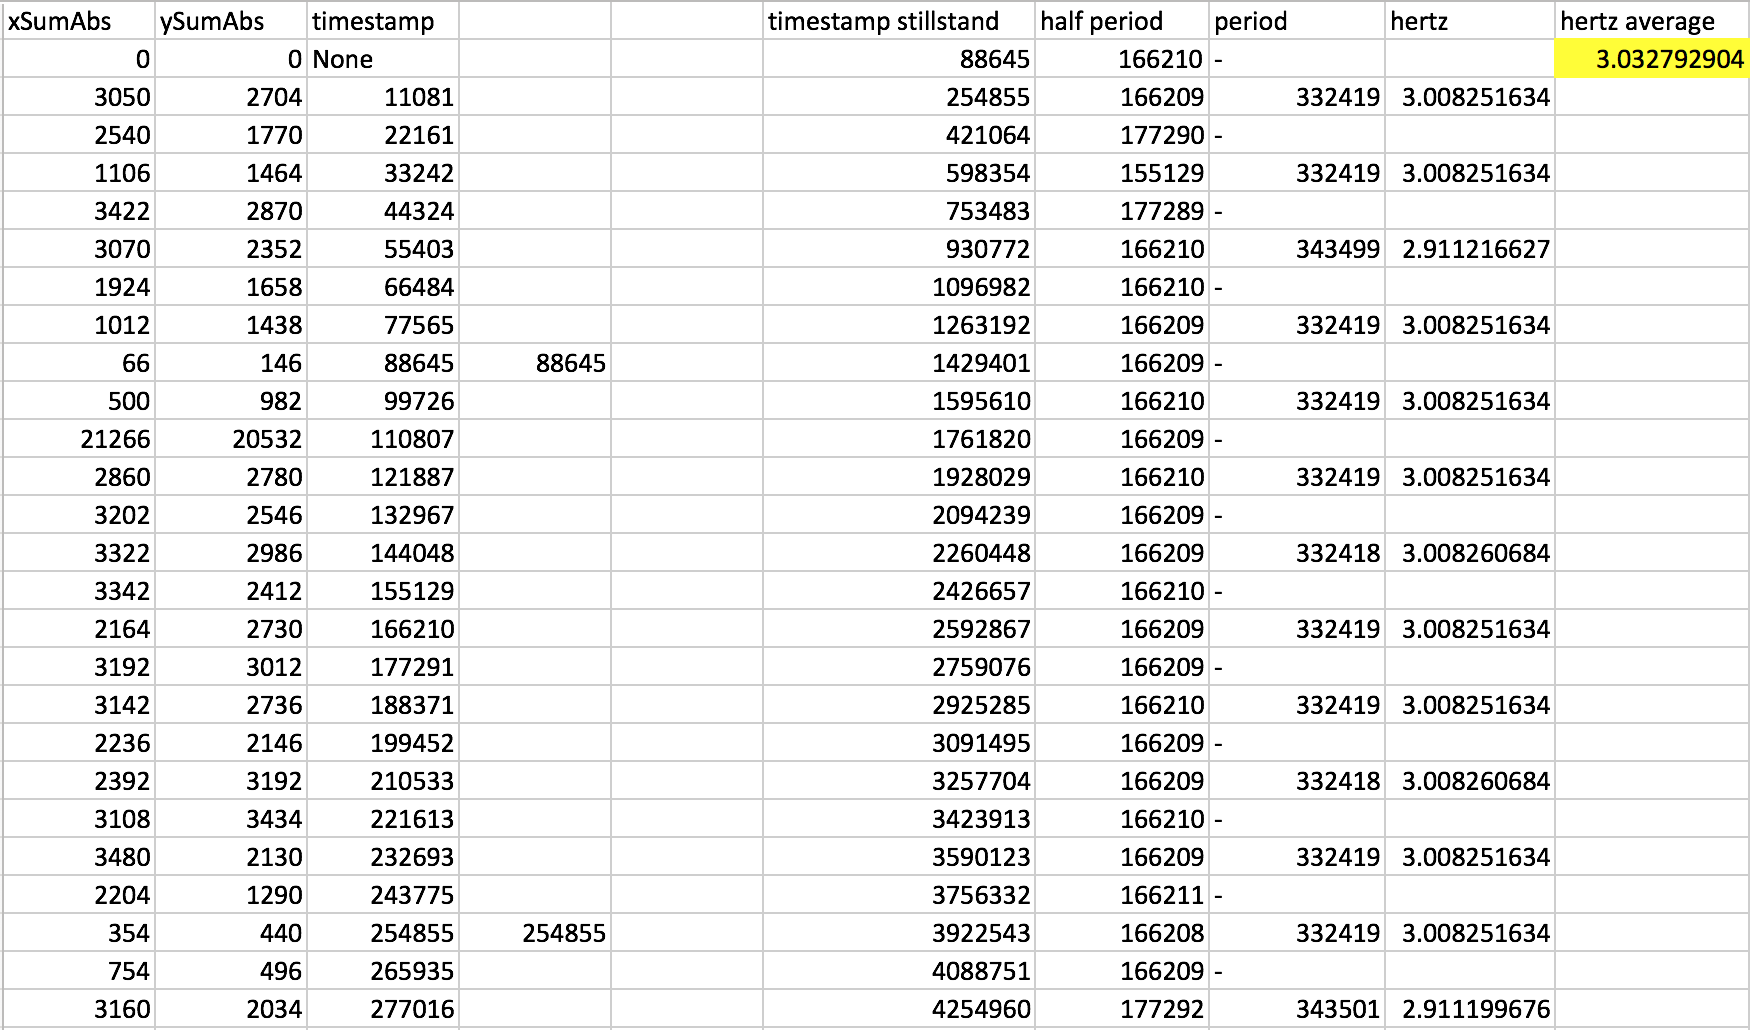
\includegraphics[scale=0.45]{Images/excel_sheet_numbers.png}
    
    \caption{Excel sheet with aggregated absolute x-, y-values, timestamps and calculated frequency}
    \end{figure}
    
    Figure 5.2 shows a graph of all aggregated absolute x-values and y-values over time and it was created out of the same excel sheet in Figure 5.1. The value over 20000 at the beginning almost always appeared, but as it does not have any impact on the measurements of the standstills of the balance wheel and only showed up at the beginning, thus it can be ignored.

    \noindent
    \begin{figure}[H]
    \centering
    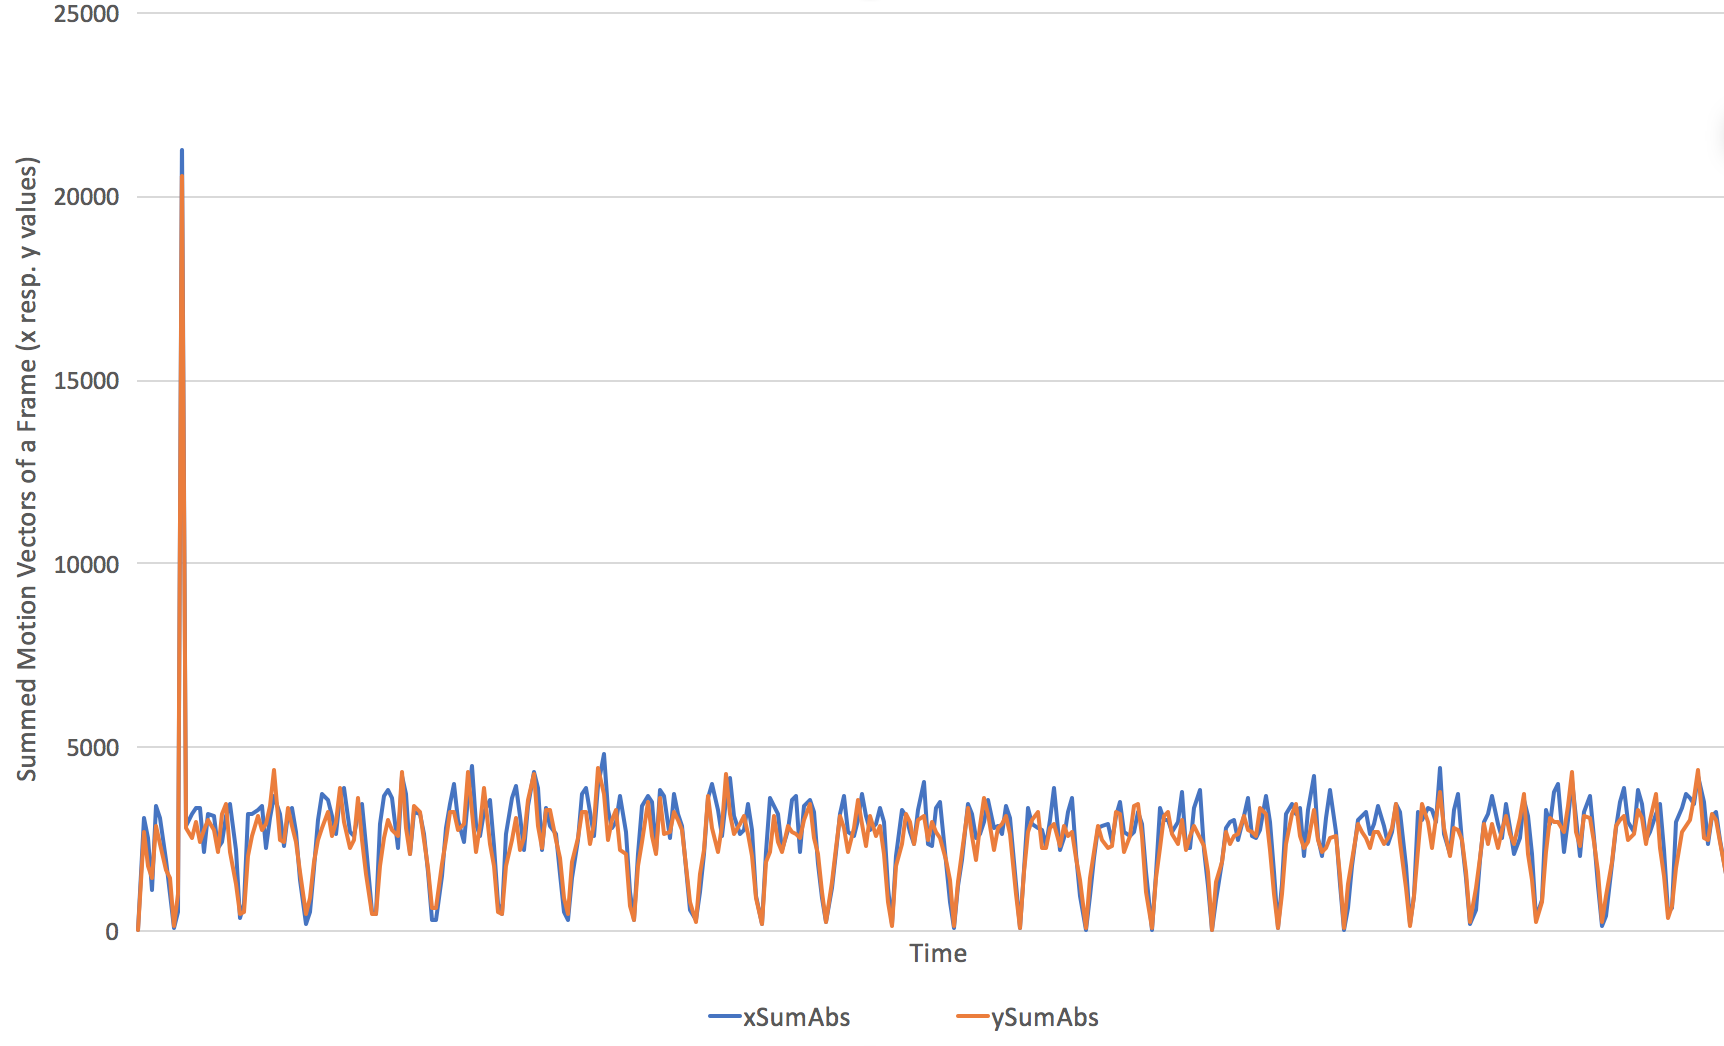
\includegraphics[scale=0.45]{Images/excel_sheet_graph.png}
    
    \caption{Illustration of aggregated summed x-(blue), y-values (red) over time. The x-axis is the time and the y-axis are the x- and y-values.}
    \end{figure}
    
       \section{Implementation of the Algorithms}
 The implementation of a Python program was based on the procedure from the Excel spreadsheet. During the first implementation, it turned out that there are different methods for calculating the frequency resulting in three different implementations each of which are explained in more detail in the following sections.
    \subsection{Counting Minima with Upper Limit} 
    
    The greatest difficulty proved to be the detection of the minimia which characterize the standstill of the balance wheel. These were relatively easy visible to the unaided eye, but for an automatic calculation, appropriate conditions had to be set in order to take into account the correct values and image noise had to be smoothed out. The setting of an upper limit for the minima proved to be a suitable condition. All minima below this limit are therefore taken into account. 
    
    Furthermore, the calculation of the frequency in the Python program has been further simplified by not calculating each period individually, but by selecting the first and the last minimum over the whole period of time in which it was recorded. This time span is then calculated by half of the number of minima minus one. Half, because every half of the period the balance wheel stops and minus one, because otherwise one half-period would be taken into account too much. This approach reduces the number of rounding errors, resulting in higher accuracy. After this calculation, the period duration $T$ is now available, from which the frequency $f$ can be calculated quite simply: 
    
     \begin{displaymath}
      f = \frac{1}{T}
     \end{displaymath}
     
  \subsection{Counting Minima with Stepsize}
  To ensure that minimas are not missed during counting, step sizes were used, that means the specifications where the minimas are to be searched for. In the measurements with the test watch, which has a stroke number of 6 per second, a frame rate of 90 was used and therefore every 15th value should show a standstill or a minimum. To detect deviations, a search window of size 5 has been defined.
  For this way, two further values are compared to the left and right of the nominal step size and 15th steps are added from the smallest value of these 5. This method does not require defining a threshold for the minima searching, which is often difficult to set. On the other hand one has to know the ideal frequency of the watch to calculate the stepsize.
  
    \subsection{Counting Minima with Tic Tac and Stepsize}
  The implementation of the program for calculating the frequency by counting the minimums with a defined step size has been adapted so that the calculation is carried out in a similar way as with the professional devices. In the previous implementation, the length of one half-period after another was measured and then the frequency was calculated. However, the semi-oscillation may differ in one direction from the semi-oscillation in the other direction, so the accuracy of the program can be improved if the length is measured from one tic to the next and exactly the same for the beat on the other side, the tac, as shown in the Figure 5.3. 
       \noindent
    \begin{figure}[H]
        \centering
        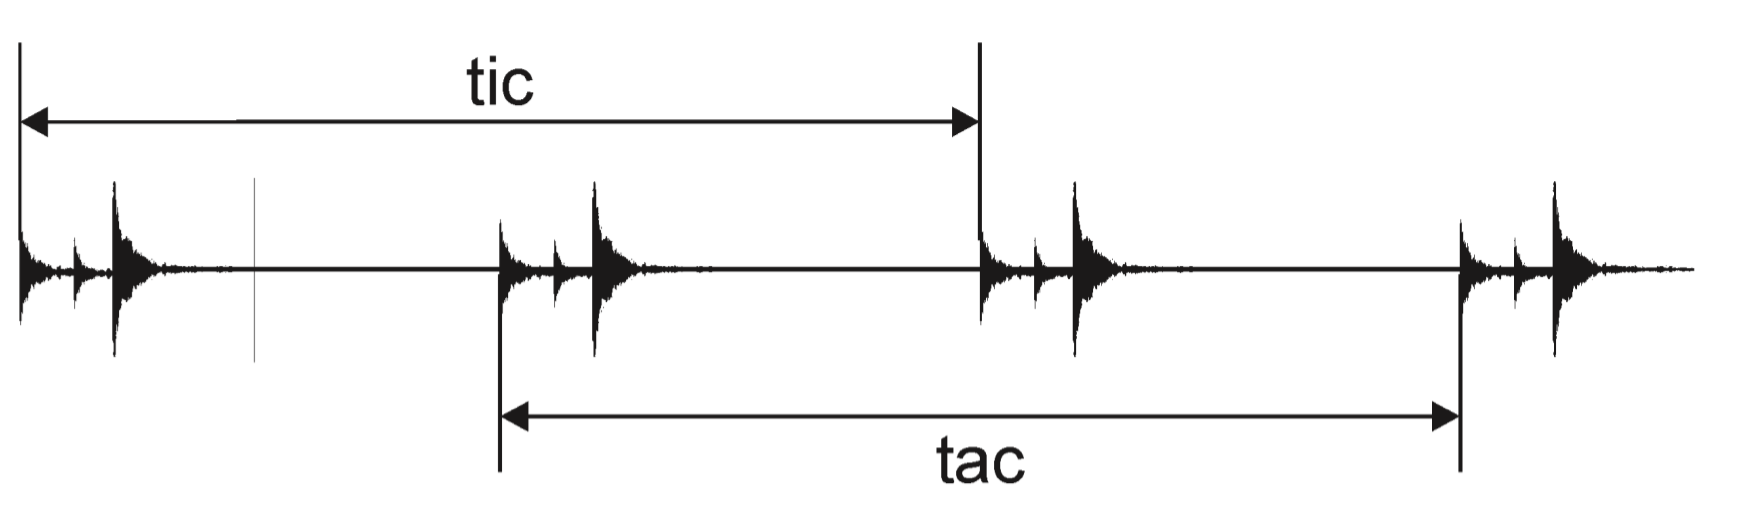
\includegraphics[scale=0.4]{Images/gangdeviation.png}
    
    \caption{Period duration of tic, i.e. tac}
    \end{figure}    
  
  This results in overlapping periods, which is why the following calculation must be carried out at the end:
  
       \begin{displaymath}
     \text{period duration} = \frac{\text{period duration of tic} + \text{period duration of tac}}{2} 
     \end{displaymath}
  and therefore: 
       \begin{displaymath}
      \text{frequency}= \frac{1}{\text{period duration}}
     \end{displaymath}
     
    
    \chapter{Results}
        The first reference measurements were performed on the test watch on three days. Two measurements were carried out with the Greiner Compact 900 and one with the Witschi Watch Expert II. Calculations using the Greiner Compact diverge greatly from those taken with the Watch Expert II. All those first measurements were not done in parallel with the camera measurements. In the first subchapter the results, this divergence and its causes will be discussed in more detail. In a next step, since the results with the first reference measurements were not useful, a verification of the accuracy of the measurements with the camera were made with a blinking LED. The last subchapter will focus on the meterings of the Greiner Compact 900 and the Raspberry Pi camera which were made in parallel and where very similiar results were obtained. 
    \section{Measurements}
As the test watch was in a distinctly colder environment (about 5 degrees Celsius) shortly before the Greiner Compact meter was used to measure the reference values, it is highly likely that the small metal spring has contracted and the watch ran faster as a result. Before the calculation with the Watch Expert II time scale, the test watch was in an ambient temperature of about 25 degrees Celsius for a long time. A difference of only 5 degrees Celsius can affect the accuracy of the watch\cite[p. 21 - 23]{Witschi_basics}. As the reference measurements are based on a difference of about 20 degrees Celsius, the above-mentioned difference occurs with the measured values obtained.
The optical measurements of the Picamera were carried out on an average at about 25 degrees Celsius, therefore the reference values determined by the Wisio Scope time scale are best suited for the comparison.

    All measurements were taken in different positions of the watch with different length
    of recordings, whereas each position was recorded during 10, 20, 40 and 80 minute intervals.
\newline

From the timestamp $t_1$ of the first stillstand and from the timestamp $t_2$ of the last timestamp, the duration $\triangle t$ of the recording can be calculated.
    \bigskip
    \begin{center}
    \(\triangle t = t_2-t_1\)
    \end{center}
     \bigskip
    
Out of this duration and the number of stillstands $n_1$, the stroke duration can be derived as follows:
    \bigskip
        \begin{center}
	\( \text{stroke duration} = \triangle t / n_1 \)
	    \end{center}
	\bigskip

Additionally, the deviation per hour is defined as 
  \bigskip
        \begin{center}
    \(\text{deviation per hour} = 3600\text{sec}-(\text{stroke duration}*n_2)\)
        
    \end{center}
        \bigskip
where $n_2$ ist the number of strokes per hour, which is 21600.

    The figure and table below show the deviation per day based on the preeceding calculation.

    \noindent
    \begin{figure}[H]
        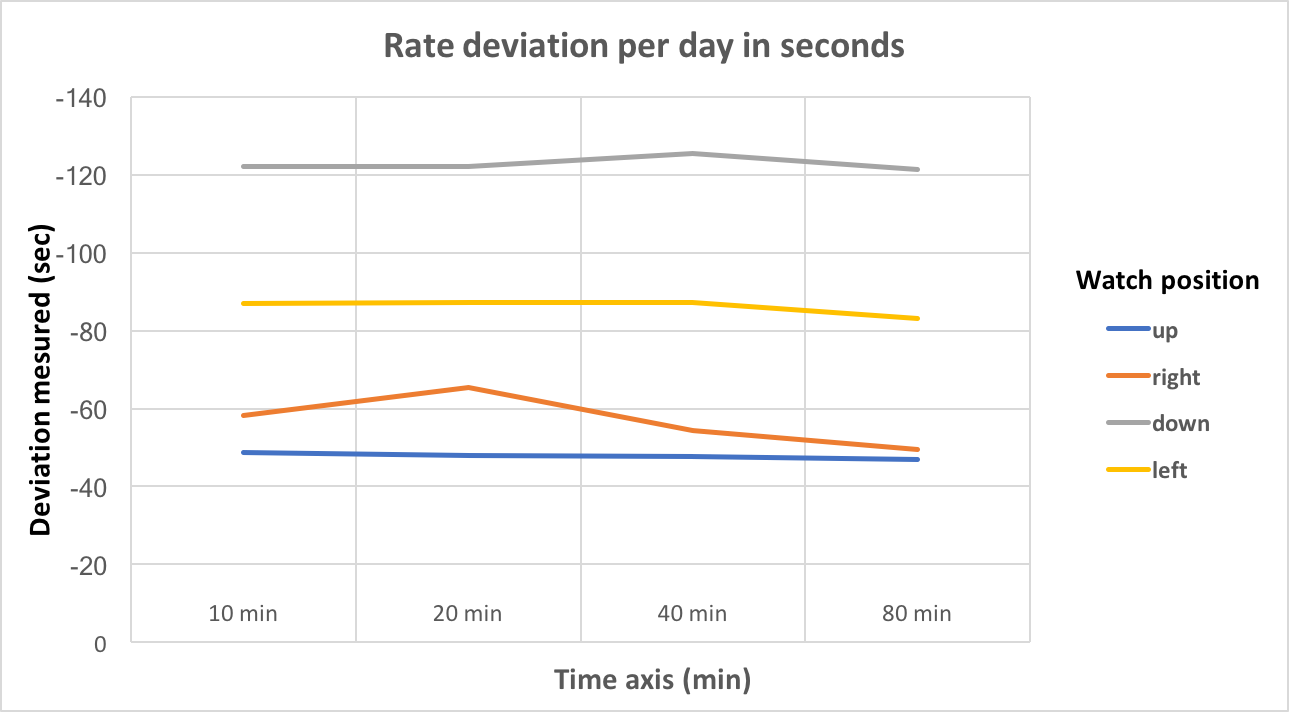
\includegraphics[scale=0.62]{Images/variations_per_day.png}
    
    \caption{ Rate deviation of different time and position recordings}
    \end{figure}    
    
    \begin{table}[H]
      \centering
        \begin{tabularx}{\linewidth}{ |X|L|L|L|L|L|L|L|L|  }
        \hline
        {\fontsize{9}{10}\selectfont \textbf{Positions}} &{\fontsize{9}{10}\selectfont \textbf{Greiner Compact 900} (first)} &{\fontsize{9}{10}\selectfont \textbf{Greiner Compact 900} (2nd)}& {\fontsize{9}{10}\selectfont \textbf{Witschi Watch Expert II}} &  \multicolumn{4}{c|}{{\fontsize{10}{12}\selectfont \textbf{Camera}}}  \\ \hline  {\fontsize{9}{10}\selectfont Metering Duration }& & & &{\fontsize{10}{12}\selectfont \textbf{10 min}} &  {\fontsize{10}{12}\selectfont \textbf{20 min}} &  {\fontsize{10}{12}\selectfont \textbf{40 min}} & {\fontsize{10}{12}\selectfont  \textbf{80 min}} \\ \hline
        up        & -13       & -17           &      -33  & -48.7     & -48.0     & -47.6      & -47.0      \\ \hline
        right     & -30        & -36        &      -62  & -58.3      & -65.5    & -54.4      & -49.4      \\ \hline
        down      & -20       & -28        &  -56  & -122.2    & -122.2     & -125.4    & -121.4      \\ \hline
        left      & -14            & -13     & -44 & -87.0	   & -87.1	  & -87.1	  & -83.1      \\ \hline
        \end{tabularx}
          \caption{ Variations per day in seconds} 
    \end{table}
    
    \section{Verification of Accuracy}
    The calculated frequency is far too imprecise. In theory, however, the calculation should become more precise after a certain period of time and should even be accurate to the microsecond.
    But this has never been achieved. For this reason, a reliable artificial clock was used in the form of an LED that is clocked by a 50 Mhz quartz and therefore is sufficiently accurate.
    
    Because trust in the motion vectors has diminished, a color-based method was used. The new method analyzes certain pixels in each image of the video sequence and detects the LED's light when a threshold value is exceeded in the RGB color space. This represents an artificial standstill of the balance wheel.
    The LED has been programmed to mimic the test watch's balance wheel and provides 21600 pulses per hour -
    respectively a frequency of 6 Hz as half periods.

    Table 6.2 shows the result of the measurements. Different durations have been selected to show the measurement becomes more accurate over time and multiple runs have been made to show that the results are reproducible.
   
    \begin{table}[H]
      \centering
        \begin{tabularx}{\linewidth}{ |L|L|L|L|L|L|  }
        \hline
        \textbf{Duration} (s) &  \textbf{run 1}  (\si\micro\/s)&  \textbf{run 2} (\si\micro\/s)&  \textbf{run 3} (\si\micro\/s)&  \textbf{run 4} (\si\micro\/s)&  \textbf{run 5} (\si\micro\/s)\\ \hline
        10        & 166591.5                 & 166585.0     & 166397.2     & 165655.4      & 166585.0      \\ \hline
        20     & 166679.0                 & 166117.1      & 166675.0    & 166675.0      & 166581.9  \\ \hline
        40      & 166486.4                 & 166673.1    & 166675.0     & 166440.3    & 166673.1    \\ \hline
        60      & 166673.7                 & 166672.4	   & 166673.7	  & 166672.4	  & 166673.7  \\ \hline
        300      & 166665.2                 & 166671.7	   & 166640.4	  & 166665.3	  & 166640.4      \\ \hline
        600      & 166668.2                 & 166649.6	   & 166668.2	  & 166655.8	  & 166668.2      \\ \hline
        900      & 166667.2                 & 166667.3	   & 166638.4	  & 166638.4	  & 166667.2      \\ \hline
        1200      & 166660.4                 & 166668.3	   & 166669.7	  & 166668.2	  & 166668.2      \\ \hline
        1500      & 166668.8                 & 166650.3	   & 166650.3	  & 166668.8	  & 166668.8      \\ \hline
        1800      & 166652.8                 & 166668.2	   & 166669.2	  & 166668.2	  & 166669.2      \\ \hline
        2100      & 166668.6                 & 166668.6	   & 166668.6	  & 166655.4	  & 166654.5      \\ \hline
        2400      & 166668.1                 & 166652.7	   & 166656.5	  & 166668.1	  & 166668.1        \\ \hline
    \end{tabularx}
    \caption{Measured impulses of led board through RGB analysis with an expected value 166666}
    \end{table}

    In Table 6.2 the assumption has been confirmed that longer records lead to more accurate measurement results.
    Surprisingly, 60 seconds of measure time already shows a close approach to the expected 166666 microseconds. The error in measurement of run 1 during 60 seconds measure time would be 3.64 seconds per day.

    \begin{figure}[H]
      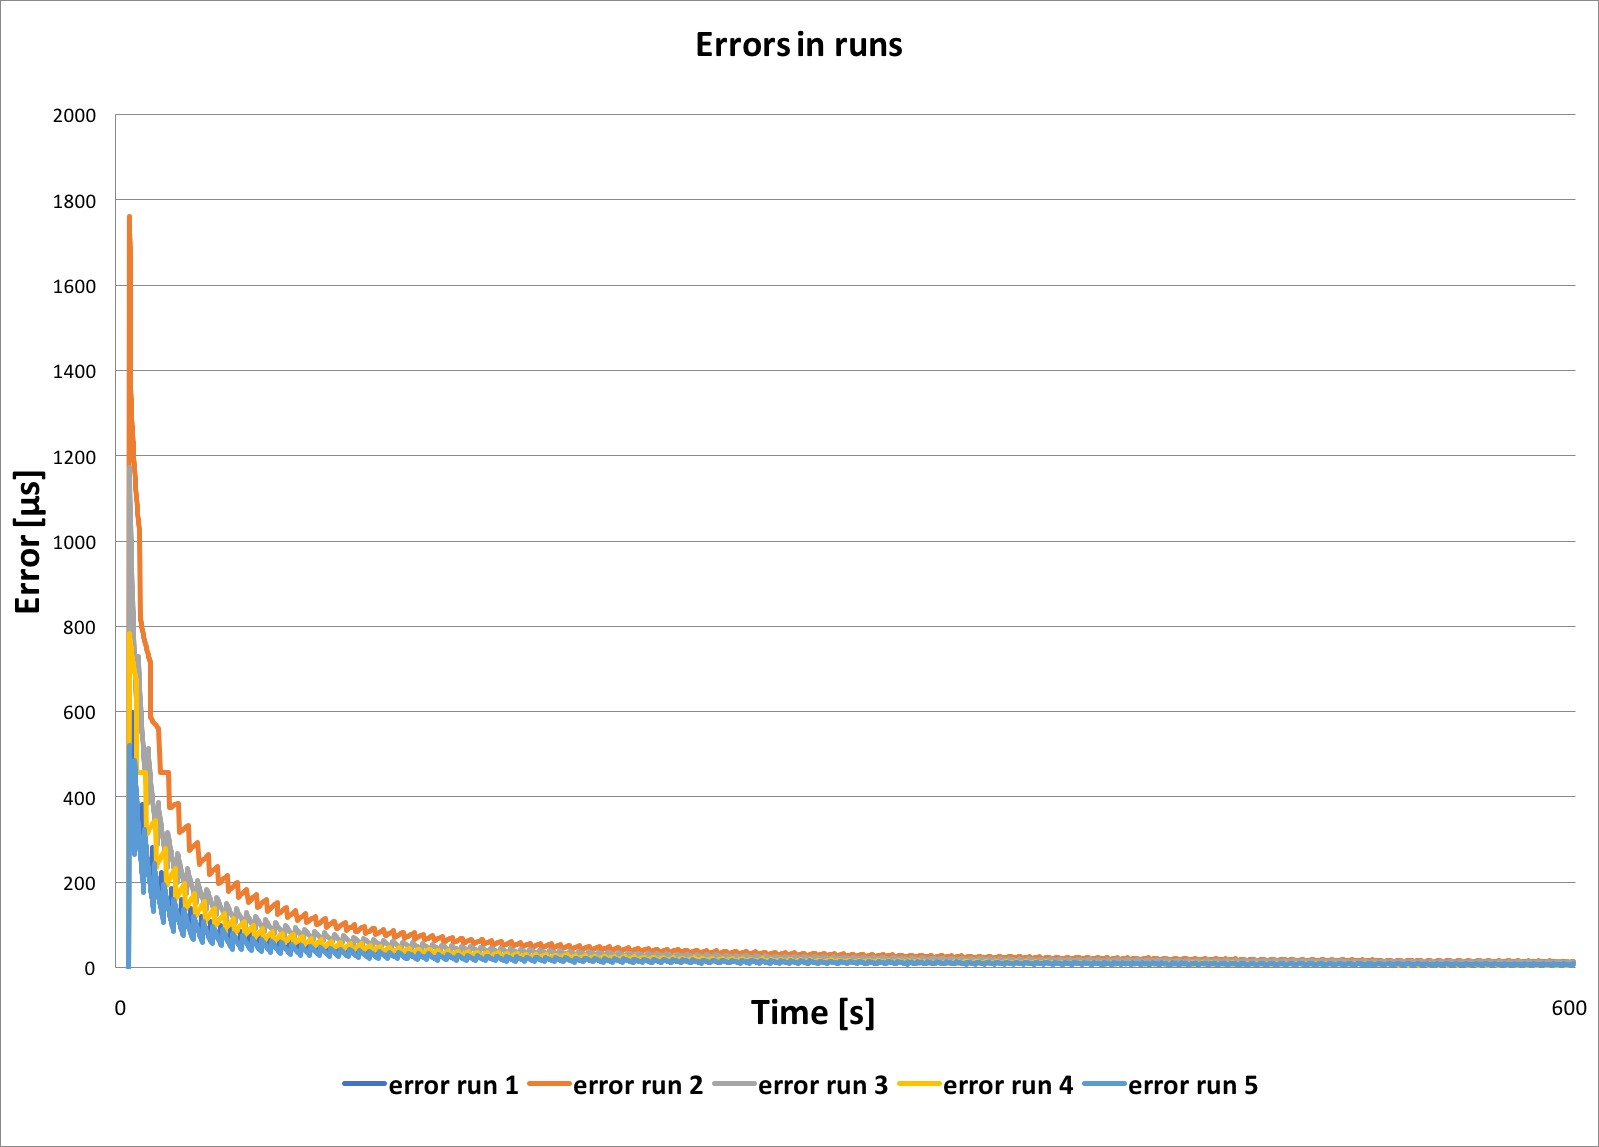
\includegraphics[scale=0.5]{Images/errors_600sec.png}
  
    \caption{Illustration of convergence of the errors}
    \end{figure}

    Figure 6.2 shows the measurement over 600 seconds and the convergence of the measurement error.
    Since exact results of the LED pulses were possible with the RGB measurement, this should also be possible with the movement vectors with additional SAD values.
    In the next measurement, instead of using RGB values, the motion vectors, i.e. the SAD values, have been used.

    \begin{table}[H]
      \centering
        \begin{tabularx}{\linewidth}{ |L|L|L|L|L|L|  }
        \hline
        \textbf{Duration} (s) &  \textbf{run 1}  (\si\micro\/s)&  \textbf{run 2} (\si\micro\/s)&  \textbf{run 3} (\si\micro\/s)&  \textbf{run 4} (\si\micro\/s)&  \textbf{run 5} (\si\micro\/s)\\ \hline
        10        & 166636.1                 & 166628.1     & 166628.1     & 166628.1      & 166628.1      \\ \hline
        20     & 166700.3                 & 166602.3      & 166700.3    & 166602.3     & 166602.3  \\ \hline
        40      & 166685.6                 & 166638.1    & 166638.1     & 166638.1    & 166638.1    \\ \hline
        60      & 166649.5                 & 166649.5	   & 166649.5	  & 166649.5	  & 166649.5  \\ \hline
        300      & 166667.4                 & 166667.4	   & 166673.6	  & 166667.4	  & 166667.4      \\ \hline
        600      & 166666.5                 & 166666.5	   & 166666.5	  & 166669.6	  & 166666.5      \\ \hline
        900      & 166668.2                 & 166666.2	   & 166668.3	  & 166668.3	  & 166651.7      \\ \hline
        1200      & 166669.1                 & 166656.7	   & 166658.3	  & 166658.4	  & 166669.3      \\ \hline
        1500      & 166669.7                 & 166659.8	   & 166658.5	  & 166669.6	  & 166659.7      \\ \hline
        1800      & 166661.7                 & 166660.7	   & 166668.9	  & 166669.9	  & 166668.9      \\ \hline
        2100      & 166668.4                 & 166661.4	   & 166668.4	  & 166669.3	  & 166662.3      \\ \hline
        2400      & 166669.7                 & 166669.6	   & 166663.5	  & 166663.5	  & 166662.7        \\ \hline
    \end{tabularx}
    \caption{Measured half periods of led board using SAD. Desired value 166666}
    \end{table}

    Table 6.3 proves that even with the SAD values accurate measurements can be made.
    This implies also the motion vectors can be used for precise measurement.

    Knowing that the methods do not only work in theory but also in practice, a metering of a Greiner Compact 900 and the Raspberry Pi camera was executed in parallel. In Figure 6.3 the setup is shown. The watch was placed on a nimble mounting of the Greiner device, which includes the microphone, that was used for measuring the oscillation of the balance wheel. 
    
      \begin{figure}[H]
        \centering
        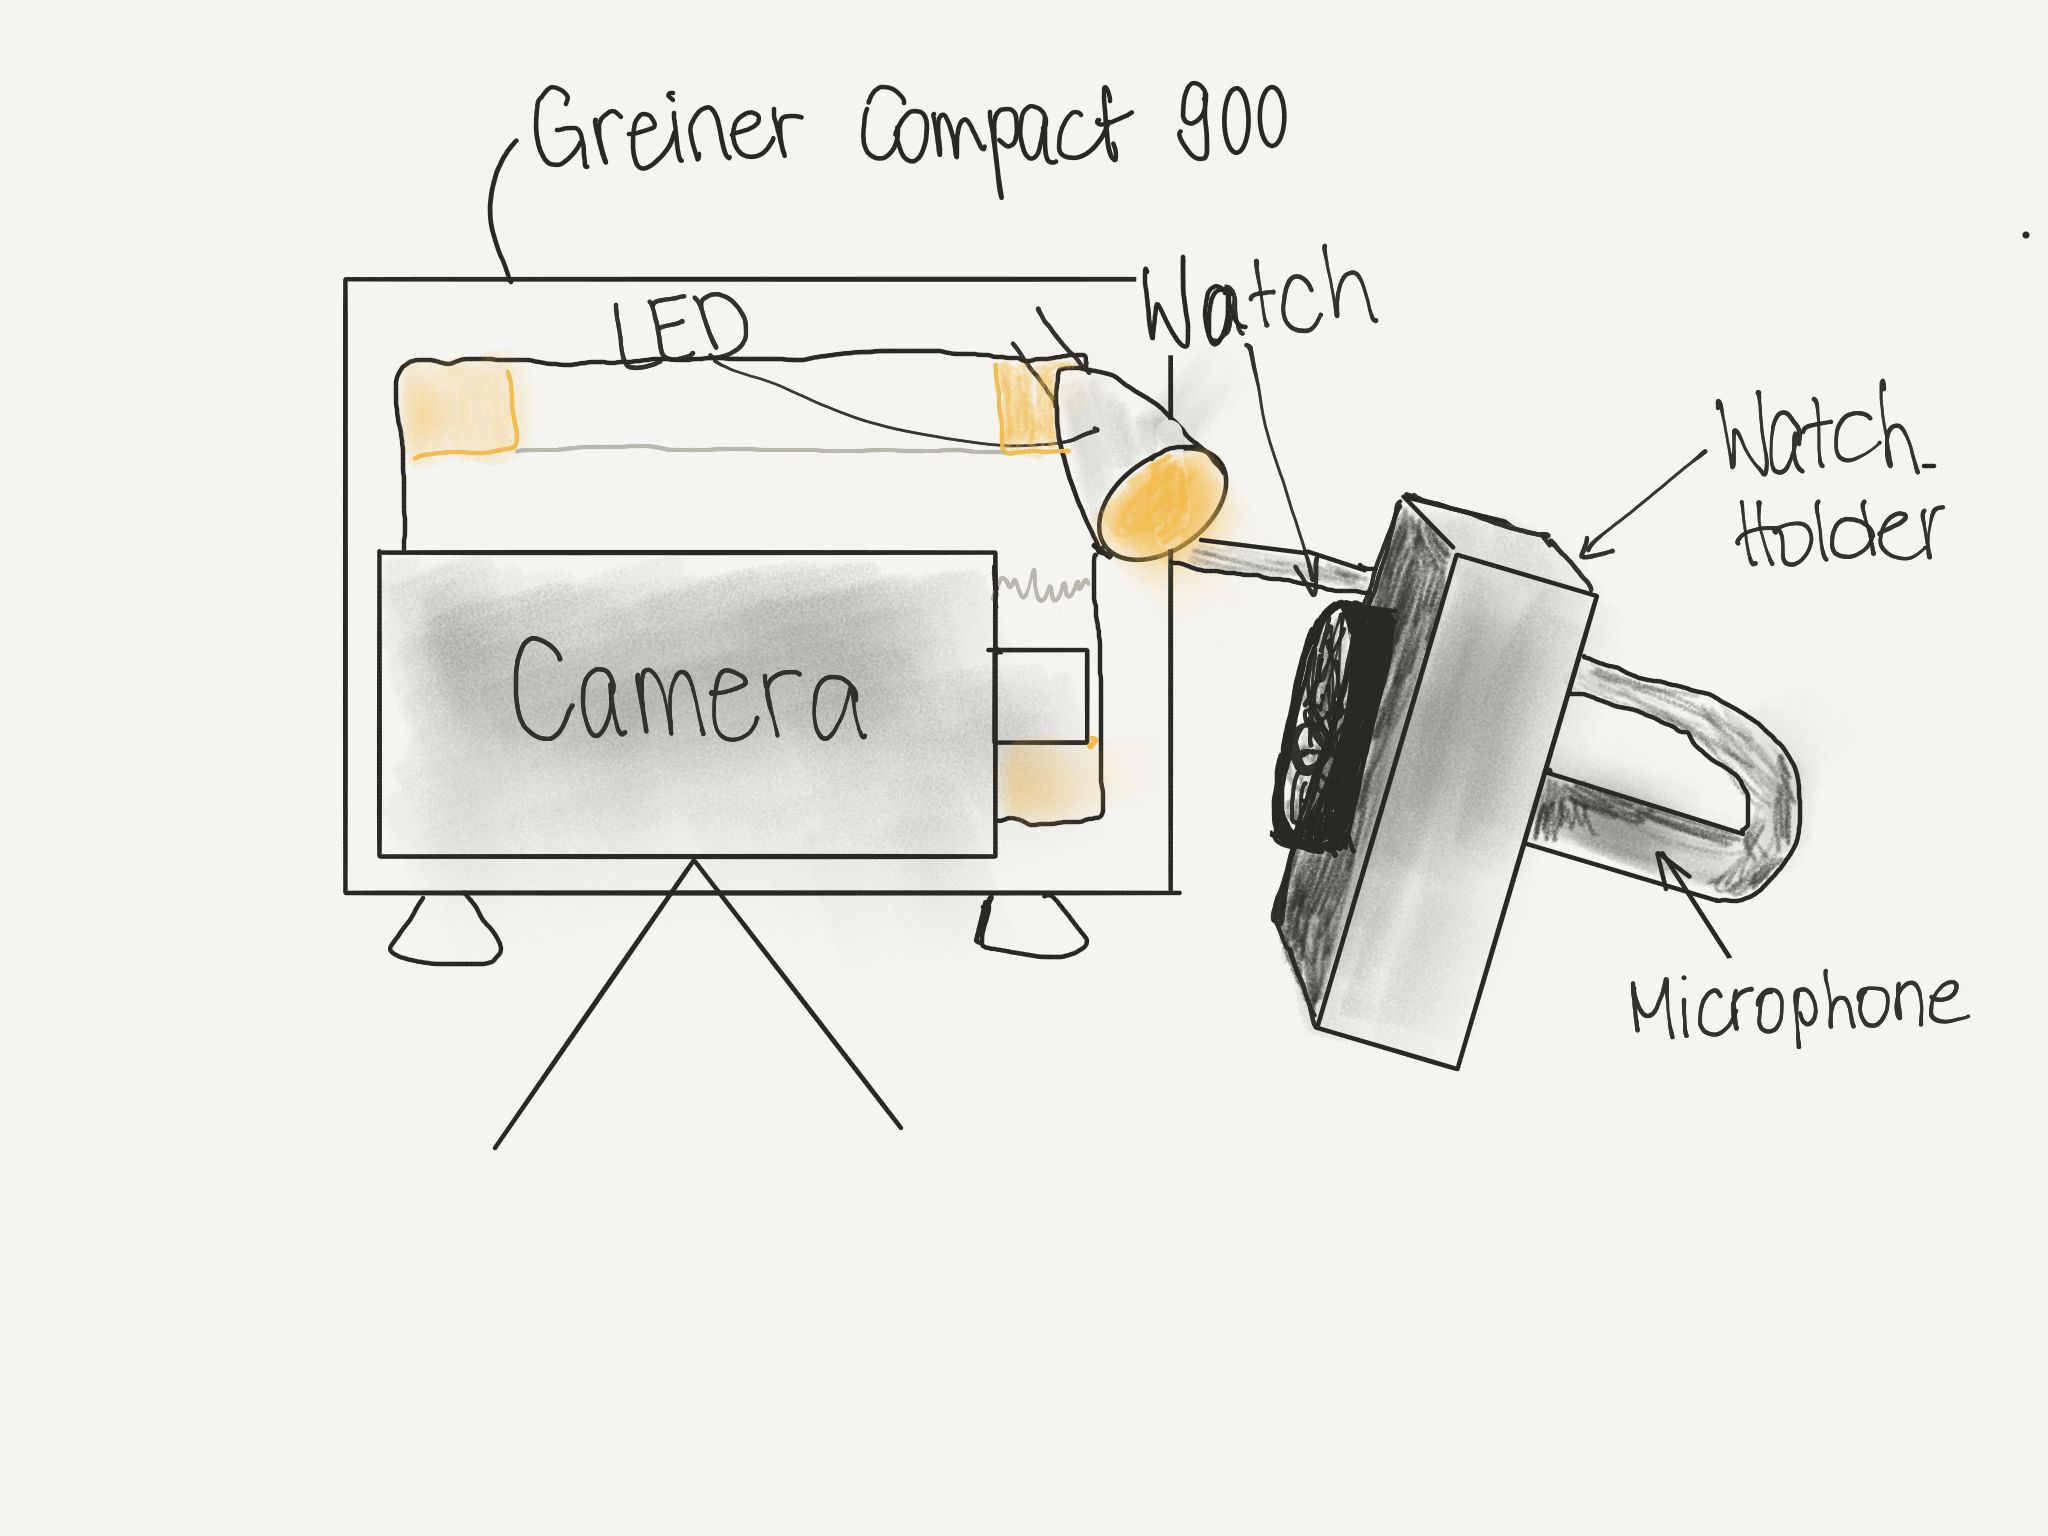
\includegraphics[scale=0.3]{Images/parallel_test_setup}
        
        \caption{Test setup for records}
        \end{figure}
        
   The oscillation of the test watch was adjusted manually seven times. Each change of this oscillation and the subsequent measurement of this new rate deviation are displayed as a row in table 6.4. 
   
   The in chapter seven introduced algorithms, "Counting Minima with Stepsize" and "Counting Minima with Tic Tac and Stepsize", were used for the calculations and compared. Both algorithms work really well, but when considering the different movement direction of the balance wheel, "tic" and "tac", the results correspond a bit more to the average of the measurements of the Greiner device.

    \begin{table}[H]
      \centering
        \begin{tabularx}{\linewidth}{ |L|L|L|  }
        \hline
         {\fontsize{9}{10}\selectfont \textbf{Greiner Compact's observed rate deviations during measurement} (s)} &  {\fontsize{9}{10}\selectfont \textbf{Camera's measured rate deviations (stepsize)} (s)} &   {\fontsize{9}{10}\selectfont \textbf{Camera's measured rate deviations (stepsize with tic tac)} (s)} \\ \hline
        -50/-52/-55        & -52.3 & -53.2\\ \hline
        -13/-14/-15        & -13.8 & -14.8\\ \hline
        -4/-5/-6          & -5.9 & -5.9\\ \hline
        0/1               & 1.1 & 0.9\\ \hline
        5/7               & 6.8 & 5.9\\ \hline
        17/19/21/         & 18.1 & 19.3\\ \hline
        43/44/45/         & 43.7 & 44.2\\ \hline
    \end{tabularx}
    \caption{Results of parallel measurement with Greiner Compact 900 and Camera}
    \end{table}

    During the measurement at Greiner, the agitation of a watch with a frequency of 2.5 Hz was measured for 600 seconds. The mode of the Greiner meter would be set to measure in an interval of 4 seconds. Correspondingly, the Greiner meter has in some cases output up to 3 different values during the 600 seconds, which are shown in Table 6.4. The camera's measurement is based on the summed y-values of the motion vectors and the minima were counted with the algorithm of 5.2.2.
    As shown in Table 6.4, the camera's measured values are very similar to those of the professional device Greiner Compact 900.
         
    \chapter{Prediction of the measurement error}
    While doing the recordings of the blinking LED and the in parallel measurement of the Greiner Compact 900 and the camera, it became apparent that the error is proportional to 1 over time. 
    To be able to make a prediction of the error of the measurement a regression over the measured values was made.
    The theoretical part of the regression will be discussed in the following section. 
    \newline
   From the approach of the regression
   
          \begin{displaymath}
      f(t)= a*\frac{1}{t}+ b
     \end{displaymath}
     
     and the values of the duration of measurement (t in s.) as well as the metered absolute measurement errors (e in s.) the regression equation for the measurement error looks as follows
     
\begin{equation}
e = A
\begin{pmatrix}
a \\ b \end{pmatrix}
 \end{equation}
 
 with 
 \begin{equation}
A = 
\begin{pmatrix}
\frac{1}{t_1} & 1\\ \vdots & \vdots \\ \frac{1}{t_n} & 1 \end{pmatrix}.
 \end{equation}
 
 To always have a quadratic matrix on the right side of the equation and therefore be able to solve it, it is multiplied with the transposed matrix of $A^T$. Thus the resulting equation is
 
 \begin{equation}
A^T e = A^T A
\begin{pmatrix}
a \\ b \end{pmatrix}
 \end{equation}
 
where $A^T e$ has the form
 \begin{equation}
A^T e = 
\begin{pmatrix}
\frac{1}{t_1}*e_1 +\frac{1}{t_2}*e_2 + \ldots + \frac{1}{t_n}*e_n \\ e_1 + e_2 + \ldots + e_n \end{pmatrix}
 \end{equation}
 
 and further 
  \begin{equation}
A^T A= 
\begin{pmatrix}
\sum_n  \frac{1}{t_i^2} & \sum_{n} \frac{1}{t_i} \\ \sum_{n} \frac{1}{t_i} & n  \end{pmatrix}.
 \end{equation}
 
 To solve the equation a Python program was implemented, which after solving it, draws a graph for the calculated $f(t)$. 
 
Figure 7.1 and Figure 7.2 which is a enlarged part of Figure 7.1 shows such a graph. The values are taken from the parallel measurement of the Greiner device and the camera when the clock had a rate deviation of about minus five seconds. As a reference value the average of the shown value of the Greiner device was taken. The calculated function for the metering error for the graph in Figure 7.1 is \( f(t) = 103.483 \frac{1}{t} + 2.209 \). 


The plot on top in Figure 7.1 are the measured values and the plot below in the same figure is drawn with the computed function. As one can easily see the graph of the calculated function matches really good with the timeline of the measured values, which proves that the error truly is proportional to 1 over time. 

      \begin{figure}[H]
        \centering
        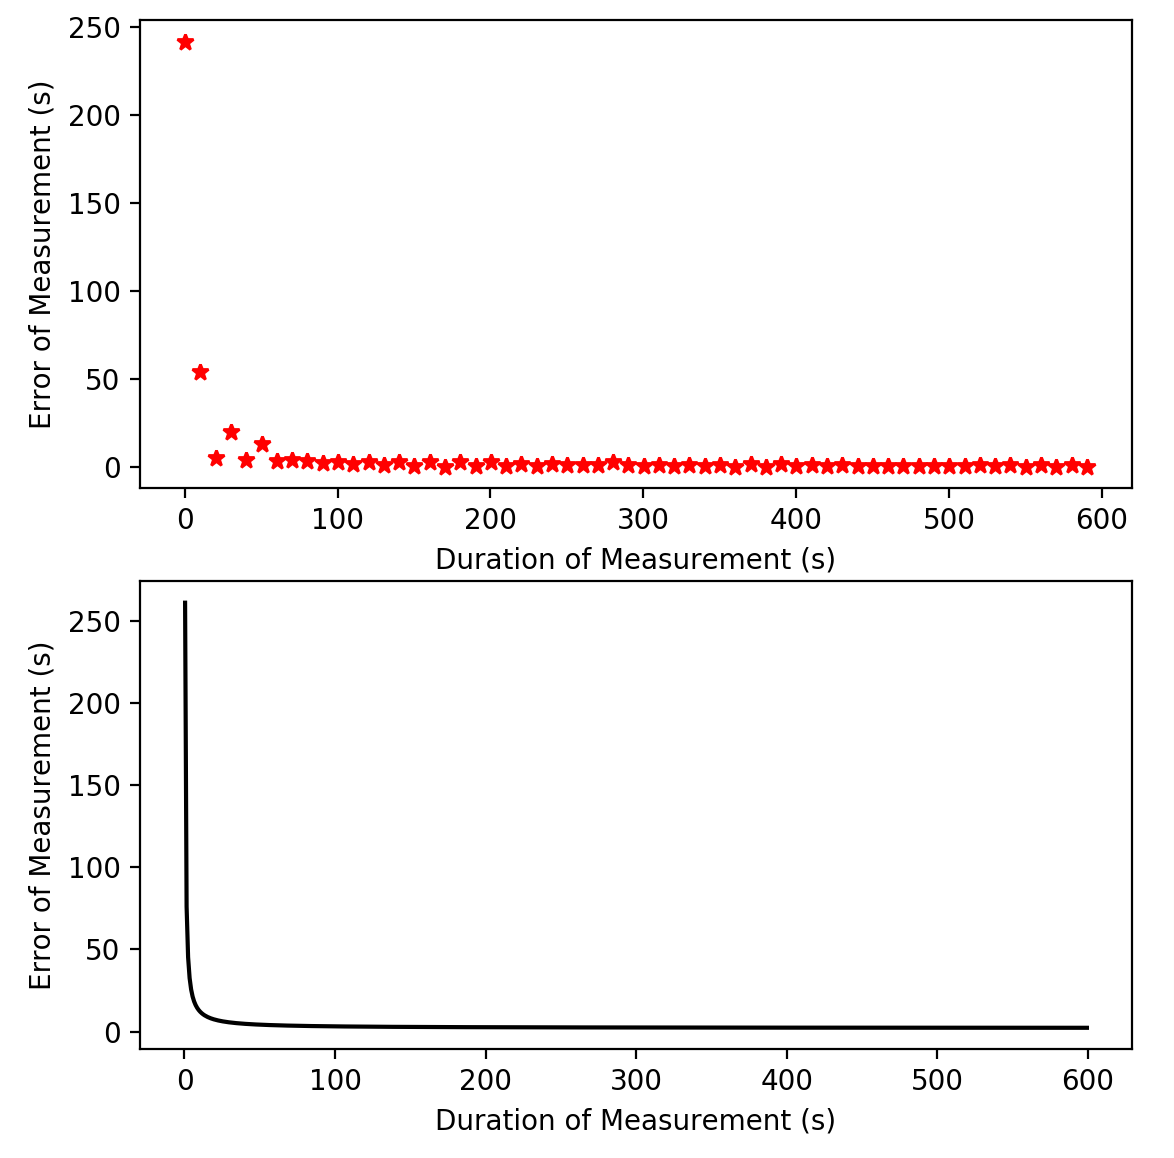
\includegraphics[scale=0.6]{Images/error_measurement}
        
        \caption{The timeline of the measurement error from recording 1s to 600s}
        \end{figure}

      \begin{figure}[H]
        \centering
        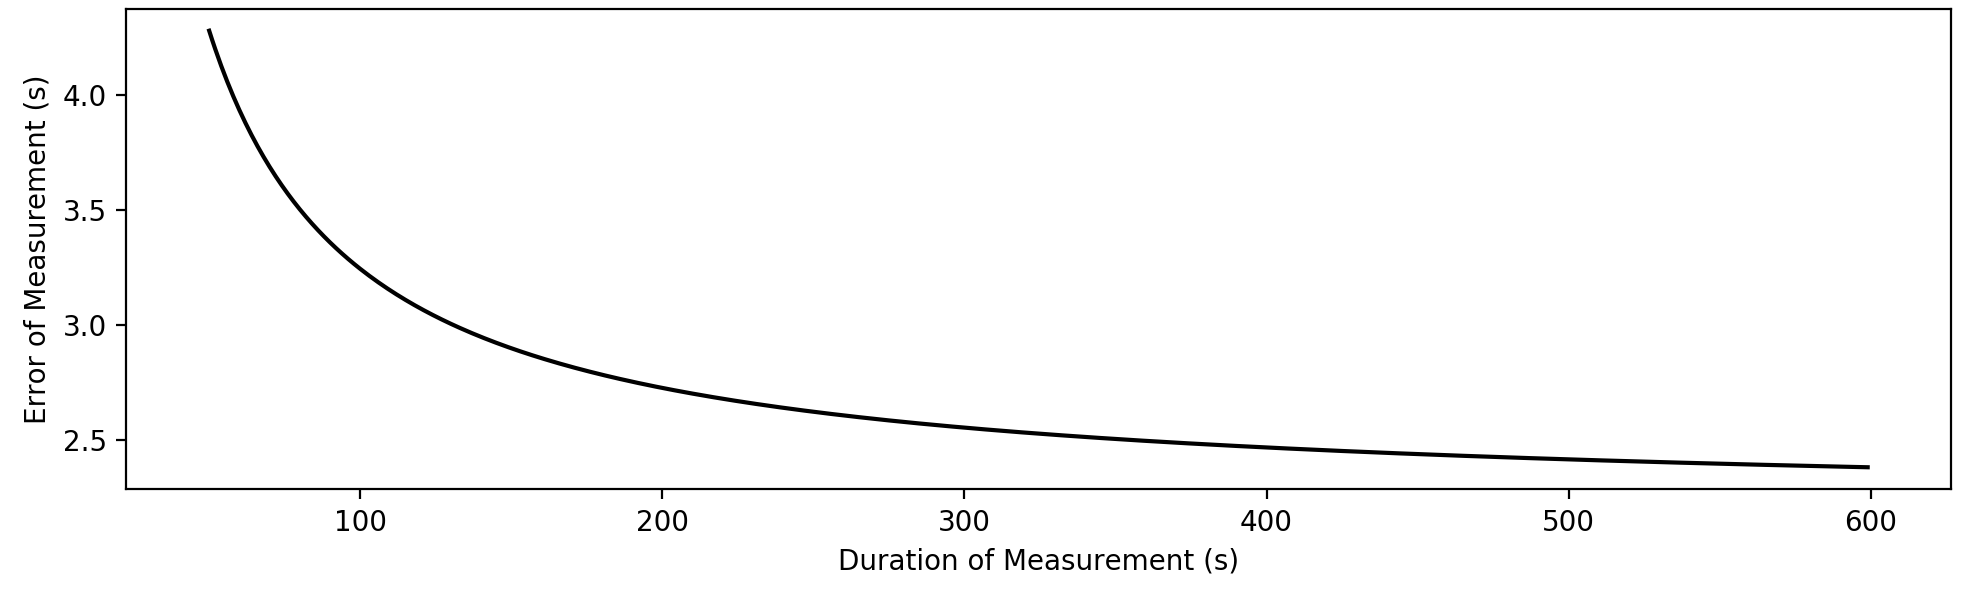
\includegraphics[scale=0.6]{Images/error_measurement_100_600}
        
        \caption{The timeline of the measurement error from recording 50s to 600s}
        \end{figure}

The determined values $a$ and $b$ were for all measurements, where the rate deviation of the watch was adjusted, more or less the same.

The calculations for $a$ were in the range of 100 to 200 and $b$ was in the range of two and four and a half. 

For example for a precision of 5, 3, and about 2s one needs 40s, 150s and 600s of measurement accordingly.

The minimal error of measurement is indicated by $b$. It appeared that there is always a minimal error of about two seconds. Compared with the Greiner Compact 900, which results fluctuate in this range as well, this is a good outcome. 
The measurements showed that after about three and a half minutes one gets an error of approximately three seconds, to lower this for another second the measurement needs to be extended up to ten minutes.     
    
    \chapter{Discussion}
    Different approaches of companies were first compared and then different algorithms and libraries for image processing were evaluated. 
    \newline
    With the help of the Picamera library and motion vectors the frequency of the balance of a mechanical watch was calculated with different implementations. Overall, the frequency was determined relatively accurate and without large deviations. Actually, all methods worked, but the implementation with the step size and the consideration of the direction of the semi-oscillation did best.
    \newline
    For the error of the measurement it was determined that it is reciprocally proportional to the measured time (see chapter 7). With this statement a forecast for the error can be made and one can distinguish how long a measurement needs to be to get the favored outcome. For a precision of 5, 3, and about 2s one needs approximately 40s, 150s and 600s of measurement accordingly. 
    \newline
    The results of image processing correlate very well with the values of professional devices. The deviation is very slight and therefore hardly weighs in. Even the results with the professional devices fluctuate slightly and so the measured values obtained in this work keep up very well with the devices. 

    \section{Difficulties}
In this work there were also some difficulties, which are specified in the following section.

The first difficulty proved to be that the standstill of the balance was easily detected by eye in the summed x- and y-values of the movement vectors, but it took a while until the Python program could reliably detect these standstills.

The right camera settings and lighting conditions turned out to be another crucial point. Especially due to too weak light, the first recordings were not usable. 

Furthermore, at the beginning too much information, i. e. complete frames, was stored on the Raspberry Pi, which caused memory overflow during measurements over 2 hours. Once this problem had been identified, only the sums of the motion vectors of a frame were stored, which saved a lot of memory.

Probably the greatest difficulty was to get good reference measurements, which could also be used as reference values. Thanks to Greiner, however, this problem could be resolved at the end by enabling parallel measurement of the professional Greiner Compact 900 and the camera.

    \section{Outlook}
    In this work it was shown that with relatively inexpensive hardware, sufficient good measurements can be carried out to determine the accuracy of a watch. Compared to the professional equipment, which costs thousands of dollars to buy, a good user interface could create a product that is much cheaper \textbf{which price?!} and can still keep up with the measurements of more expensive devices. 
 To get a device, which can compete with the professional ones however some additional measurements for other information of the watch need to be implemented. Almost all watch metering devices on the market are able to adjust the lifting angle of the watch, which can have an impact on the oscillation of the balance wheel. Something different that sure needs to be further implemented is the amplitude, which corresponds to the angle of rest position of the balance wheel until turning point. When those things are implemented, the camera will be ready for the market. 
    
    \glsaddall
    \printglossaries

\addcontentsline{toc}{chapter}{Bibliography}
\printbibliography
        
    \addcontentsline{toc}{chapter}{List of Figures}    
    \listoffigures
    \bigskip
      
    
    \end{document}